\chapter{Results}
\label{ch:results}
	\note{IN PROGRESS}

	\section{Deforestation}
	\label{sec:results_deforestation}

		\subsection{Forest definition}
		\label{subsec:results_forest_definition}
		%TODO appendix graph distribution of the similarity indexes
		%TODO review
			\note{Goal (review):} Our goal was to determine at which canopy cover class the similarity between both layers is greatest to get the subsequent proximate deforestation driver for stable land cover changes optimal by anthropogenic causes by keeping the largest number of pixels from the gfc dataset. We applied the jaccard index for searching the similarity. We grouped our analysis by continental regions americas, asia, africa. Americas accounts for 82 tiles, Asia 86 tiles and Africa 101. We excluded from the analysis all tiles where the initial jaccard index is zero because theses tiles does not contain any tree cover in both tile pairs. This results in 76 Americas , 73 asia and 86 africa. Further we determined the optimal canopy density class for all regions and for single regions by applying the non parametric two and one sided wilcoxon signed rank test. Our initial hypothesis was that the agreement is max between gl30 and hansen when the selected canopy density is between 30 and 100. Because then both datasets should agree by their authors definition of tree cover. The following paragraphs present the results of the analysis for each continental region. 

			\note{Americas (review):} Figure \ref{fig:jaccard} shows the quartile distribution of the computed jaccard index for each tile pair for each canopy density class over the three continental regions. Plotted on the x-axis is the canopy density class identifier where $JI_0$ accounts for (0,100], $JI_0$ (10,100], $JI_0$ (20,100], and $JI_0$ (30,100]. The y-axis is the corresponding jaccard index between 0 and 1 for the corresponding tile pair where 1 means total agreement and 0 total disagreement. The sample mean highlight by red crosses in the boxplot for the Americas does not change significantly within the different canopy density classes. For all experiments it is approximately 0.62. While the sample median decreases from 0.68 to 0.66 from the first canopy density class the last canopy density class. For the first canopy class the upper 25 \% of the samples have tree cover similarity ranging between approximately 0.8 and 1.0. This behavior can be observed at the other canopy density classes to only the maximal similarity increases slightly from 0.9787 to 0.9798. As the figure \note{appendix} suggests the change of the canopy density have only little impact on the tiles where already the similarity is high for the upper 25 percent. The similarity range of the first two canopy density classes for the lower 25 percent of the samples ranges between approximately 0.0003 and 0.47. Whereas the range for last to canopy classes ranges between 0.0 and 0.5. This suggests that the exclusion of higher canopy densities decreases the similarity at samples where the similarity is already low also shown in figure \note{appendix}. 50 percent of the samples have a jaccard index between approximately 0.5 and 0.8 where here the highest mobility of similarity increase and decrease can be observed. To deduce which canopy density class yield the highest similarity in the distribution overall all samples from americas we applied a wilcoxon test. Tabel \ref{tab:wilcoxontwosided_regions} and \ref{tab:wilcoxontwosided_regions} shows the results from these tests. The two sided test reveals that only the similarity distribution between $JI_0$ and $JI_1$ has a significant (p<0.01) difference in distribution. The other Jaccard Index pairs show now significant difference in distribution. The tree cover similarity distribution of $JC_1$ is significantly greater than $JC_0$ (p<0.005) as the results from the one sided test show in the second table. Therefore the exclusion of canopy densities < 11 fosters the overall agreement between both tree cover datasets. Further the test also reveals that the similarity distribution of $JC_2$ is significantly greater than $JC_1$ (p<0.05) but by the comparison of $JC_1$ and $JC_2$ shows no clear trend in a certain direction. It is to assume that $JC_2$ improves only the tree cover agreement for certain tile pairs and not in general. The same accounts for $JC_3$. For studies targeting Americas it is to recommended to use from the Global Forest Change dataset data which lays within the canopy densities greater than 10 percent.
			\begin{figure}[ht]
				\centering
				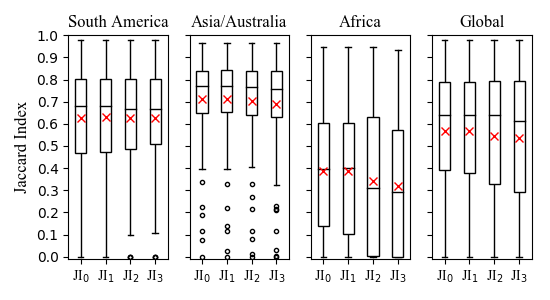
\includegraphics[scale=.91]{img/jaccard}
				\caption[Tree cover similarity distribution of the continental regions]{\textbf{Tree cover similarity distribution over the continental regions:} This boxplot shows the distribution of computed Jaccard Index for each raster image tile pair of GlobeLand30 and Global Forest Change tree cover from 2000. The labels $JI_0$, $JI_1$, $JI_2$, and $JI_3$ on the x-axis account for the canopy density classes (0,100], (10,100], (20,100], and (30,100], respectively. The y-axis is the computed Jaccard Index for the corresponding raster image pair, where 0 is a total disagreement and 1 a total agreement. Red crosses within the $Q_{25}$, $Q_{50}$, and $Q_{75}$ boxes highlight the sample mean. Whiskers are 1.5 times the $IQR$.}
				\label{fig:jaccard}
			\end{figure}
			\begin{table}[ht]
				\centering
				\caption[Regional two-sided Wilcoxon signed-rank test]{\textbf{Regional two-sided Wilcoxon signed-rank test:} This table shows, regional differences in the tree cover agreement by considering different canopy densities between GlobeLand30 and Global Forest Change at 2000. The classes $JI_0$, $JI_1$, $JI_2$, and $JI_3$ as row and column headings account for the canopy density classes (0,100], (10,100], (20,100], and (30,100], respectively. The test hypothesis is H$_0$: $X_1=X_2$ where $X_1$ is the column $JI_n$ class and $X_2$ the row $JI_n$ class. The significance is indicated by $p^{*}<0.05$, $p^{**}<0.02$, and $p^{***}<0.01$.}
				\label{tab:wilcoxontwosided_regions}
				\begin{tabular}{llllllllll}
					\hline
					& \multicolumn{3}{|c}{Americas} & \multicolumn{3}{|c|}{Asia} & \multicolumn{3}{c|}{Africa} \\
					Cls & JI$_0$ & JI$_1$ & JI$_2$ & JI$_0$ & JI$_1$ & JI$_2$ & JI$_0$ & JI$_1$ & JI$_2$ \\\hline
					JI$_0$ & - & - & - & - & - & - & - & - & - \\
					JI$_1$ & .00$^{***}$ & - & - & .72 & - & - & .22 & - & - \\
					JI$_2$ & .06 & .36 & - & .00$^{***}$ & .00$^{***}$ & - & .03$^{*}$ & .03$^{*}$  & - \\
					JI$_3$ & .16 & .50 & .60 & .00$^{***}$ & .00$^{***}$ & .00$^{***}$ & .00$^{***}$ & .00$^{***}$ & .00$^{***}$ \\\hline
				\end{tabular}
			\end{table}
			\begin{table}[ht]
				\centering
				\caption[Regional one-sided Wilcoxon signed-rank test]{\textbf{Regional one-sided Wilcoxon signed-rank test:} This table shows, the direction of regional differences in the tree cover agreement by considering different canopy densities between GlobeLand30 and Global Forest Change at 2000. The classes $JI_0$, $JI_1$, $JI_2$, and $JI_3$ as row and column headings account for the canopy density classes (0,100], (10,100], (20,100], and (30,100], respectively. The test hypothesis is H$_0$: $X_1\leq X_2$ and H$_0$: $X_2\geq X_1$ where $X_1$ is the column $JI_n$ class and $X_2$ the row $JI_n$ class. The significance is indicated by $p^{*}<0.05$, $p^{**}<0.025$, $p^{***}<0.01$, and $p^{\dagger}<0.005$.}
				\label{tab:wilcoxononesided_regions}
				\begin{tabular}{lllllllllllll}
					\hline
					& \multicolumn{4}{|c}{Americas} & \multicolumn{4}{|c|}{Asia} & \multicolumn{4}{c|}{Africa} \\
					Cls & JI$_0$ & JI$_1$ & JI$_2$ & JI$_3$ & JI$_0$ & JI$_1$ & JI$_2$ & JI$_3$ & JI$_0$ & JI$_1$ & JI$_2$ & JI$_3$ \\\hline
					JI$_0$ & - & .00$^{\dagger}$ & .03$^{*}$ & .08 & - & .64 & 1. & 1. & - & .11 & .98 & 1. \\
					JI$_1$ & 1. & - & .18 & .25 & .36 & - & 1. & 1. & .89 & - & .99 & 1. \\
					JI$_2$ & .97 & .82 & - & .30 & .00$^{\dagger}$ & .00$^{\dagger}$ & - & 1. & .02$^{**}$ & .01$^{**}$ & - & 1. \\
					JI$_3$ & .92 & .75 & .70 & - & .00$^{\dagger}$ & .00$^{\dagger}$ & .00$^{\dagger}$ & - & .00$^{\dagger}$ & .00$^{\dagger}$ & .00$^{\dagger}$ & - \\\hline
				\end{tabular}
			\end{table}
 
			\note{Asia (review):} As figure \ref{fig:jaccard} suggest does the sample mean is approximately 0.7 for all canopy classes in asia. It decreases slightly at higher canopy density intervals. The median is approximately 0.8 by showing also a slight decrease when the canopy density class is raised. The similarity of the upper 25 percent of the samples is approximately 0.85 and 0.96 and the maximum similarity decreases slightly from 0.9654 to 0.9634 by increasing canopy density interval. This suggests as the appendix figure shows that high ranking tiles are not largely impacted by changes in the canopy density. For Asia the range of the lower 25 percent of the samples is quite large. It ranges between approximately 0.65 and 0.0 and as appendix shows the mobility of the samples show an overall downward trend. The iqr for the first two canopy density classes ranges between 0.65 and 0.85. The exclusion of lower canopy densities have not an large impact on the distribution of tree cover similarity. For last two canopy density classes the range between q1 and q3 is increasing. The exclusion of higher canopy densities leads to overall downwards trend within this intervals figure appendix. For asia the two sided wilcoxon test in table \ref{tab:wilcoxontwosided_regions} reveals that the similarity distribution between every sample pair is significantly different (p<0.01) except the pair of $JI_1$ and $JI_0$. The directional test in table \ref{tab:wilcoxononesided_regions} shows that the overall tree cover agreement of $JI_2$ and $JI_3$ is significantly smaller than $JI_0$ and $JI_1$ (p<0.005). The direction of distribution differences between $JC_0$ and $JC_1$ is not clearly deduce able. This could be explained over a large variability within regional tree cover agreement also a clearer picture could be achieved by applying smaller canopy density exclusion stepping. For studies in asia it is to recommended to use from the Global Forest Change dataset data which lays within the canopy densities greater than 10 percent or the entire data range. Here it must be decided if moving the canopy density threshold below the GlobaLand30 forest cover definition is a good trade for increased sample size.

			\note{Africa (review):} As figure \ref{fig:jaccard} for Africa suggests is the similarity distribution mobility of the samples in Africa at highest. The first two similarity distributions have an comparable mean and median at 0.38 and 0.4. The last two classes show a strong decline in mean and median to approximately 0.33 and 0.3. The mobility of the upper 25 percent of the first two canopy density classes is already quite strong as figure appendix suggests. While the iqr range for $JI_0$ is between 0.15 and 0.6 the range increases for the second $JI_1$ by connecting to more agreement downwards trend. The tile pairs in africa are characterized by 17 (approx. 20 percent) where the tree cover agreement is smaller than 0.1. 11 of these tiles have already a agreement of 0.0 when the first canopy density is excluded. These trend continues as more canopy density is excluded as more samples have a agreement of 0.0. This explains the high iqr range for the canopy densities exclusion greater than 10 percent. At $JI_3$ already two fifth (42 percent) of the samples have an tree cover agreement lower than 0.1. The two sided wilcoxon test shows that the distribution of $JI_2$ and $JI_3$ significantly differs (p<0.05 and p<0.01). As the table suggest is the distribution of $JI_0$ and $JI_1$ nearly the same. The one sided test reveals that reducing the canopy density below 10 percent decreases the tree cover agreement between sample distributions. For $JI_0$ and the $JI_1$ the test reveals that no clear trend is detectable. Appendix figure shows that some samples benefit from the exclusion of canopy density and as mentioned some samples show a strong decrease in tree cover similarity. As the data shows is the regional dependency of tree cover agreement at largest. To maximize the similarity on continental level for africa it should the entire data range of Global Forest Change should be slected. It could also be also a solution to select canopy densities in the interval 10 to 100 but here the trade is to have tiles where no tree cover agreement is detectable.

			\note{Comparison between regions (review):} Table appendix shows that Asia has the highest tree cover similarity distribution over all regions within all tested canopy classes followed by the Americas for GlobeLand30 and Hansen 2000. Africa has the poorest tree cover agreement within our tested regions. As discussed in the previous paragraphs the reason could be that Americas and Asia have mainly core tropical forest zones where the forest cover is dense and the canopy density is above 30 percent. This can be highlighted by section tropical deforestation and the shown tree cover maps. Africa in comparison to Asia and Americas has large zones where the tree cover is high but the canopy density is low also described by the term sparse woodland. As it looks these sparse woodlands compete the forest detection methods of both datasets. This fact could lead within the hansen dataset to ghost deforestation because it is hard to detect sparse woodland it could be the annual deforestation does not detect it as forest and it is recognized as deforestation. Therefore in africa the rationality of tree cover agreement must be considered during preparation and validation of studies. Also it is to suggest to optimize tree cover agreement on regional scale and not over the entire continent. Overall regions the upper 25 percent of the samples benefit or shown only small changes if the canopy density is increased.

			\note{All regions (review):} To deduce in which canopy density interval we use the Global Forest Change data for our global study on proximate deforestation driver we analyzed the change of tree cover agreement over all samples. Figure \ref{fig:jaccard} shows on the right hand side of the image the distribution of tree cover agreement over the entire sample range. The mean and median shown only a slight decline overall canopy density test classes. As deduced for the regions also on global scale the upper 25 percent commonly benefit or show no change if the canopy density is increased. As the figure shows is the range of them between 0.8 and 1.0. When the canopy density is increased the range of the mid 50 percent increases which highlights a more similarity downwards trend within this group. This downwards trend of the mid is connected with a decrease in the range of the lower 25 percent. The first canopy density class is between 0.4 and 0.0 and the last is between 0.3 ad 0.0. The distribution comparison in table \ref{tab:wilcoxontwosided_all} shows that each sample class has significant differences (p<0.02 and p<0.01) except $JI_0$ and $JI_2$ where the similarity distribution could be the same. Table \ref{tab:wilcoxononesided_all} shows the direction of the distribution differences. Globally the tree cover agreement is highest when we consider only pixels within the canopy density interval (10,100] as the table shows. The distributions of tree cover agreement of $JI_0$, $JI_2$, and $JI_3$ are all significantly smaller than $JI_1$ (p<0.005 and p<0.01). By knowing this we decided to proceed for our study only with data within this tree cover interval. Therefore we filtered forest loss and gain of Global Forest Change to lay in this interval and classified them subsequently by superimposing the GlobeLand30 land cover layer. The result of this process are shown in section \ref{subsec:results_proxy_deforestation_driver}.
			\begin{table}[ht]
				\centering
				\caption[Global two-sided Wilcoxon signed-rank test]{\textbf{Regional two-sided Wilcoxon signed-rank test:} This table shows, global differences in the tree cover agreement by considering different canopy densities between GlobeLand30 and Global Forest Change at 2000. The classes $JI_0$, $JI_1$, $JI_2$, and $JI_3$ as row and column headings account for the canopy density classes (0,100], (10,100], (20,100], and (30,100], respectively. The test hypothesis is H$_0$: $X_1=X_2$ where $X_1$ is the column $JI_n$ class and $X_2$ the row $JI_n$ class. The significance is indicated by $p^{*}<0.05$, $p^{**}<0.02$, and $p^{***}<0.01$.}
				\label{tab:wilcoxontwosided_all}
				\begin{tabular}{llll}
					\hline
					Cls & JI$_0$ & JI$_1$ & JI$_2$ \\\hline
					JI$_0$ & - & - & - \\
					JI$_1$ & .00$^{***}$ & - & - \\
					JI$_2$ & .08 & .02$^{**}$ & - \\
					JI$_3$ & .00$^{***}$ & .00$^{***}$ & .00$^{***}$ \\\hline
				\end{tabular}
			\end{table}
			\begin{table}[ht]
				\centering
				\caption[Global one-sided Wilcoxon signed-rank test]{\textbf{Global one-sided Wilcoxon signed-rank test:} This table shows, the direction of global differences in the tree cover agreement by considering different canopy densities between GlobeLand30 and Global Forest Change at 2000. The classes $JI_0$, $JI_1$, $JI_2$, and $JI_3$ as row and column headings account for the canopy density classes (0,100], (10,100], (20,100], and (30,100], respectively. The test hypothesis is H$_0$: $X_1\leq X_2$ and H$_0$: $X_2\geq X_1$ where $X_1$ is the column $JI_n$ class and $X_2$ the row $JI_n$ class. The significance is indicated by $p^{*}<0.05$, $p^{**}<0.025$, $p^{***}<0.01$, and $p^{\dagger}<0.005$.}
				\label{tab:wilcoxononesided_all}
				\begin{tabular}{lllll}
					\hline
					Cls & JI$_0$ & JI$_1$ & JI$_2$ & JI$_3$ \\\hline
					JI$_0$ & - & .00$^{****}$ & .96 & 1. \\
					JI$_1$ & 1. & - & .99 & 1. \\
					JI$_2$ & .04$^{*}$ & .01$^{***}$ & - & 1. \\
					JI$_3$ & .00$^{****}$ & .00$^{****}$ & .00$^{****}$ & - \\\hline
				\end{tabular}
			\end{table}

		\subsection{Tree cover and deforestation}
		\label{subsec:results_tree_cover_and_deforestation}
		%TODO images of loss and canopy
		\note{Goal:}
		\note{Americas:} \note{Asia:} \note{Africa:}

		\subsection{Proximate deforestation driver}
		\label{subsec:results_proxy_deforestation_driver}

		\subsection{Accuracy assessment}
		\label{subsec:results_accuracy_assessment}
		%TODO distribution is it in line with global estimates
			\note{Goal (review):} Goal is the assessment of the accuracy of our proximate deforestation driver predictions. We created a set of ground truth data by sampling our proximate deforestation driver layers. In each region we select per random 10 tiles and draw 200 samples per tile. The 200 samples comprises pixels over the full value range of our proximate deforestation driver classes. We imported the prepared sample to our JavaScript application and subsequently classified each sample with a label. To determine the accuracy we used a confusion matrix and the derived metrics like producers accuracy, overall accuracy, kappa coefficient etc.

			\note{Results (review):} Table \ref{tab:results_confusion_matrix} shows the confusion matrix to determine the accuracy of our predictions where the term reference refers to the labeling of pixel by our visual interpretation and predictions refer to the labeling of our proximate driver predictions. The abbreviations PAc, UAc, OvAc, Com, Om, Tot, and Kappa refer to the terms Producers-Accuracy, Users-Accuracy, Overall-Accuracy, Error of Commission, Error of Omission, row or column total, and Kappa Coefficient. From the 6000 samples we draw from our study extent 14 \%, 20 \%, 22 \%, 32 \%, 8 \%, 2 \%, 0.5 \%, 2 \%, and 0.5 \% account for cultivated land (10), tree cover (20), regrowth (25), shrubland (40), wetland (50), water (60), artificial land (80), and bareland (90), respectively. The method predicts a distribution of 15 \%, 18 \%, 27 \%, 31 \%, 7 \%, 1 \%, 0.8 \%, 1 \%, and 0.2 \% for the land cover classes 10, 20, 25, 30, 40, 50, 60, 80, and 90, respectively. Our method achieved an overall accuracy of approximately 76 \%

			\begin{itemize}
				\item grassland in majority with anthropogenic influence at many sides at water hole was detectable
				\item decision between regrowth and natural tree cover, relayed on expert knowledge how homogeneous is canopy
				\item shrub land comprises natural landscapes, young plantations, and areas for cattle ranching
				\item strong variability of images some high res some landsat quality
			\end{itemize}
			\begin{table}[ht]
				\centering
				\caption[Confussion matrix]{\textbf{Confussion matrix for accuracy assessment:} We draw 6000 samples from 10 random selected tiles from the three regions Americas, Asia and Africa. Labels refer to our proximate deforestation driver classes which correspond to GlobeLand30 classification schema in table \ref{tab:gl30_classes}. Reference refers to the samples we classified by visual interpretation of external imagery and predictions refer to the label the sample has in our proximate driver product. The abbreviations PAc, UAc, OvAc, Com, Om, Tot, and Kappa refer to the terms Producers-Accuracy, Users-Accuracy, Overall-Accuracy, Error of Commission, Error of Omission, row or column total, and Kappa Coefficient.}
				\label{tab:results_confusion_matrix}
				\begin{tabular}{llrrrrrrrrrrrr}
					\hline
					& & \multicolumn{9}{c}{Reference} & & & \\\cline{3-11}
					& Cls & 10 & 20 & 25 & 30 & 40 & 50 & 60 & 80 & 90 & Tot & UAc & Om \\\hline
					\multirow{9}{*}{\STAB{\rotatebox[origin=c]{90}{Prediction}}}
					& 10 & 730 & 37 & 62 & 15 & 16 & 2 & 3 & 5 & 0 & 870 & .84 & .16 \\ 
					& 20 & 41 & 744 & 56 & 189 & 31 & 12 & 0 & 15 & 4 & 1092 & .68 & .32 \\ 
					& 25 & 29 & 202 & 1155 & 172 & 22 & 10 & 5 & 11 & 4 & 1610 & .72 & .28 \\ 
					& 30 & 36 & 187 & 32 & 1466 & 73 & 21 & 0 & 17 & 0 & 1832 & .80 & .20 \\ 
					& 40 & 14 & 21 & 4 & 41 & 352 & 1 & 1 & 2 & 1 & 437 & .81 & .19 \\ 
					& 50 & 0 & 5 & 3 & 10 & 4 & 50 & 0 & 1 & 0 & 73 & .68 & .32 \\ 
					& 60 & 2 & 1 & 0 & 3 & 0 & 2 & 18 & 2 & 0 & 28 & .64 & .36 \\ 
					& 80 & 3 & 3 & 0 & 1 & 1 & 1 & 0 & 40 & 0 & 49 & .82 & .18 \\ 
					& 90 & 0 & 0 & 0 & 1 & 0 & 0 & 0 & 3 & 5 & 9 & .56 & .44 \\\hline 
					& Tot & 855 & 1200 & 1312 & 1898 & 499 & 99 & 27 & 96 & 14 & 6000 & & \\
					& PAc & .85 & .62 & .88 & .77 & .71 & .51 & .67 & .42 & .36 & Kappa & \multicolumn{2}{r}{OvAc} \\
					& Com & .15 & .38 & .12 & .23 & .29 & .49 & .33 & .58 & .64 & .69 & \multicolumn{2}{r}{.76} \\ \hline
				\end{tabular}
			\end{table}

	\section{Emissions}

	\section{Ecosystem service values}




%%%%%%% TABLE AND FIGURES

%			\begin{table}[ht]
%				\centering
%				\caption[Deforestation driver]{Absolute in km$^2$}
%				\label{tab:driver_tab}
%				\begin{tabular}{lcllrrr}
%					Class & Code & Type & & Americas & Asia & Africa \\\hline
%					\multirow{4}{*}{Agriculture} & \multirow{2}{*}{10} & \multirow{2}{*}{Cropland} & rel. & 24.37 & 18.37 & 25.01 \\
%					& & & abs. & 95908 & 38719 & 44368 \\
%					& \multirow{2}{*}{30} & \multirow{2}{*}{Grassland} & rel. & 46.19 & 8.41 & 50.46 \\
%					& & & abs. & 181781 & 17726 & 89516 \\
%					\multirow{4}{*}{Forestry/Plantations} & \multirow{2}{*}{25} & \multirow{2}{*}{Regrowth} & rel. & 14.40 & 70.27 & 18.61 \\
%					& & & abs. & 56671 & 148111 & 33014 \\
%					& \multirow{2}{*}{40} & \multirow{2}{*}{Shrubland} & rel. & 12.69 & 1.11 & 3.77 \\
%					& & & abs. & 49941 & 2340 & 6688 \\
%					\multirow{4}{*}{Urban/Mining} & \multirow{2}{*}{80} & \multirow{2}{*}{Artificial} & rel. & 0.41 & 0.46 & 0.71 \\
%					& & & abs. & 1614 & 970 & 1260 \\
%					& \multirow{2}{*}{90} & \multirow{2}{*}{Bareland} & rel. & 0.10 & 0.03 & 0.09 \\
%					& & & abs. & 394 & 63 & 160 \\
%					\multirow{4}{*}{Natural} & \multirow{2}{*}{50} & \multirow{2}{*}{Wetland} & rel. & 1.50 & 0.97 & 1.23 \\
%					& & & abs. & 5903 & 2045 & 2182 \\
%					& \multirow{2}{*}{60} & \multirow{2}{*}{Water} & rel. & 0.32 & 0.38 & 0.13 \\
%					& & & abs. & 1259 & 801 & 231 \\\hline
%					\multicolumn{3}{c}{\multirow{2}{*}{Forest loss}} & rel. & 3.87 & 4.68 & 1.69 \\
%					& & & abs. & 393550 & 210774 & 177400 \\
%					\multicolumn{3}{c}{Forest cover} & abs. & 10223187 & 4457940 & 10496591 \\\hline
%				\end{tabular}
%			\end{table}

% LATIN AMERICA
%			\begin{figure}[ht]
%				\centering
%				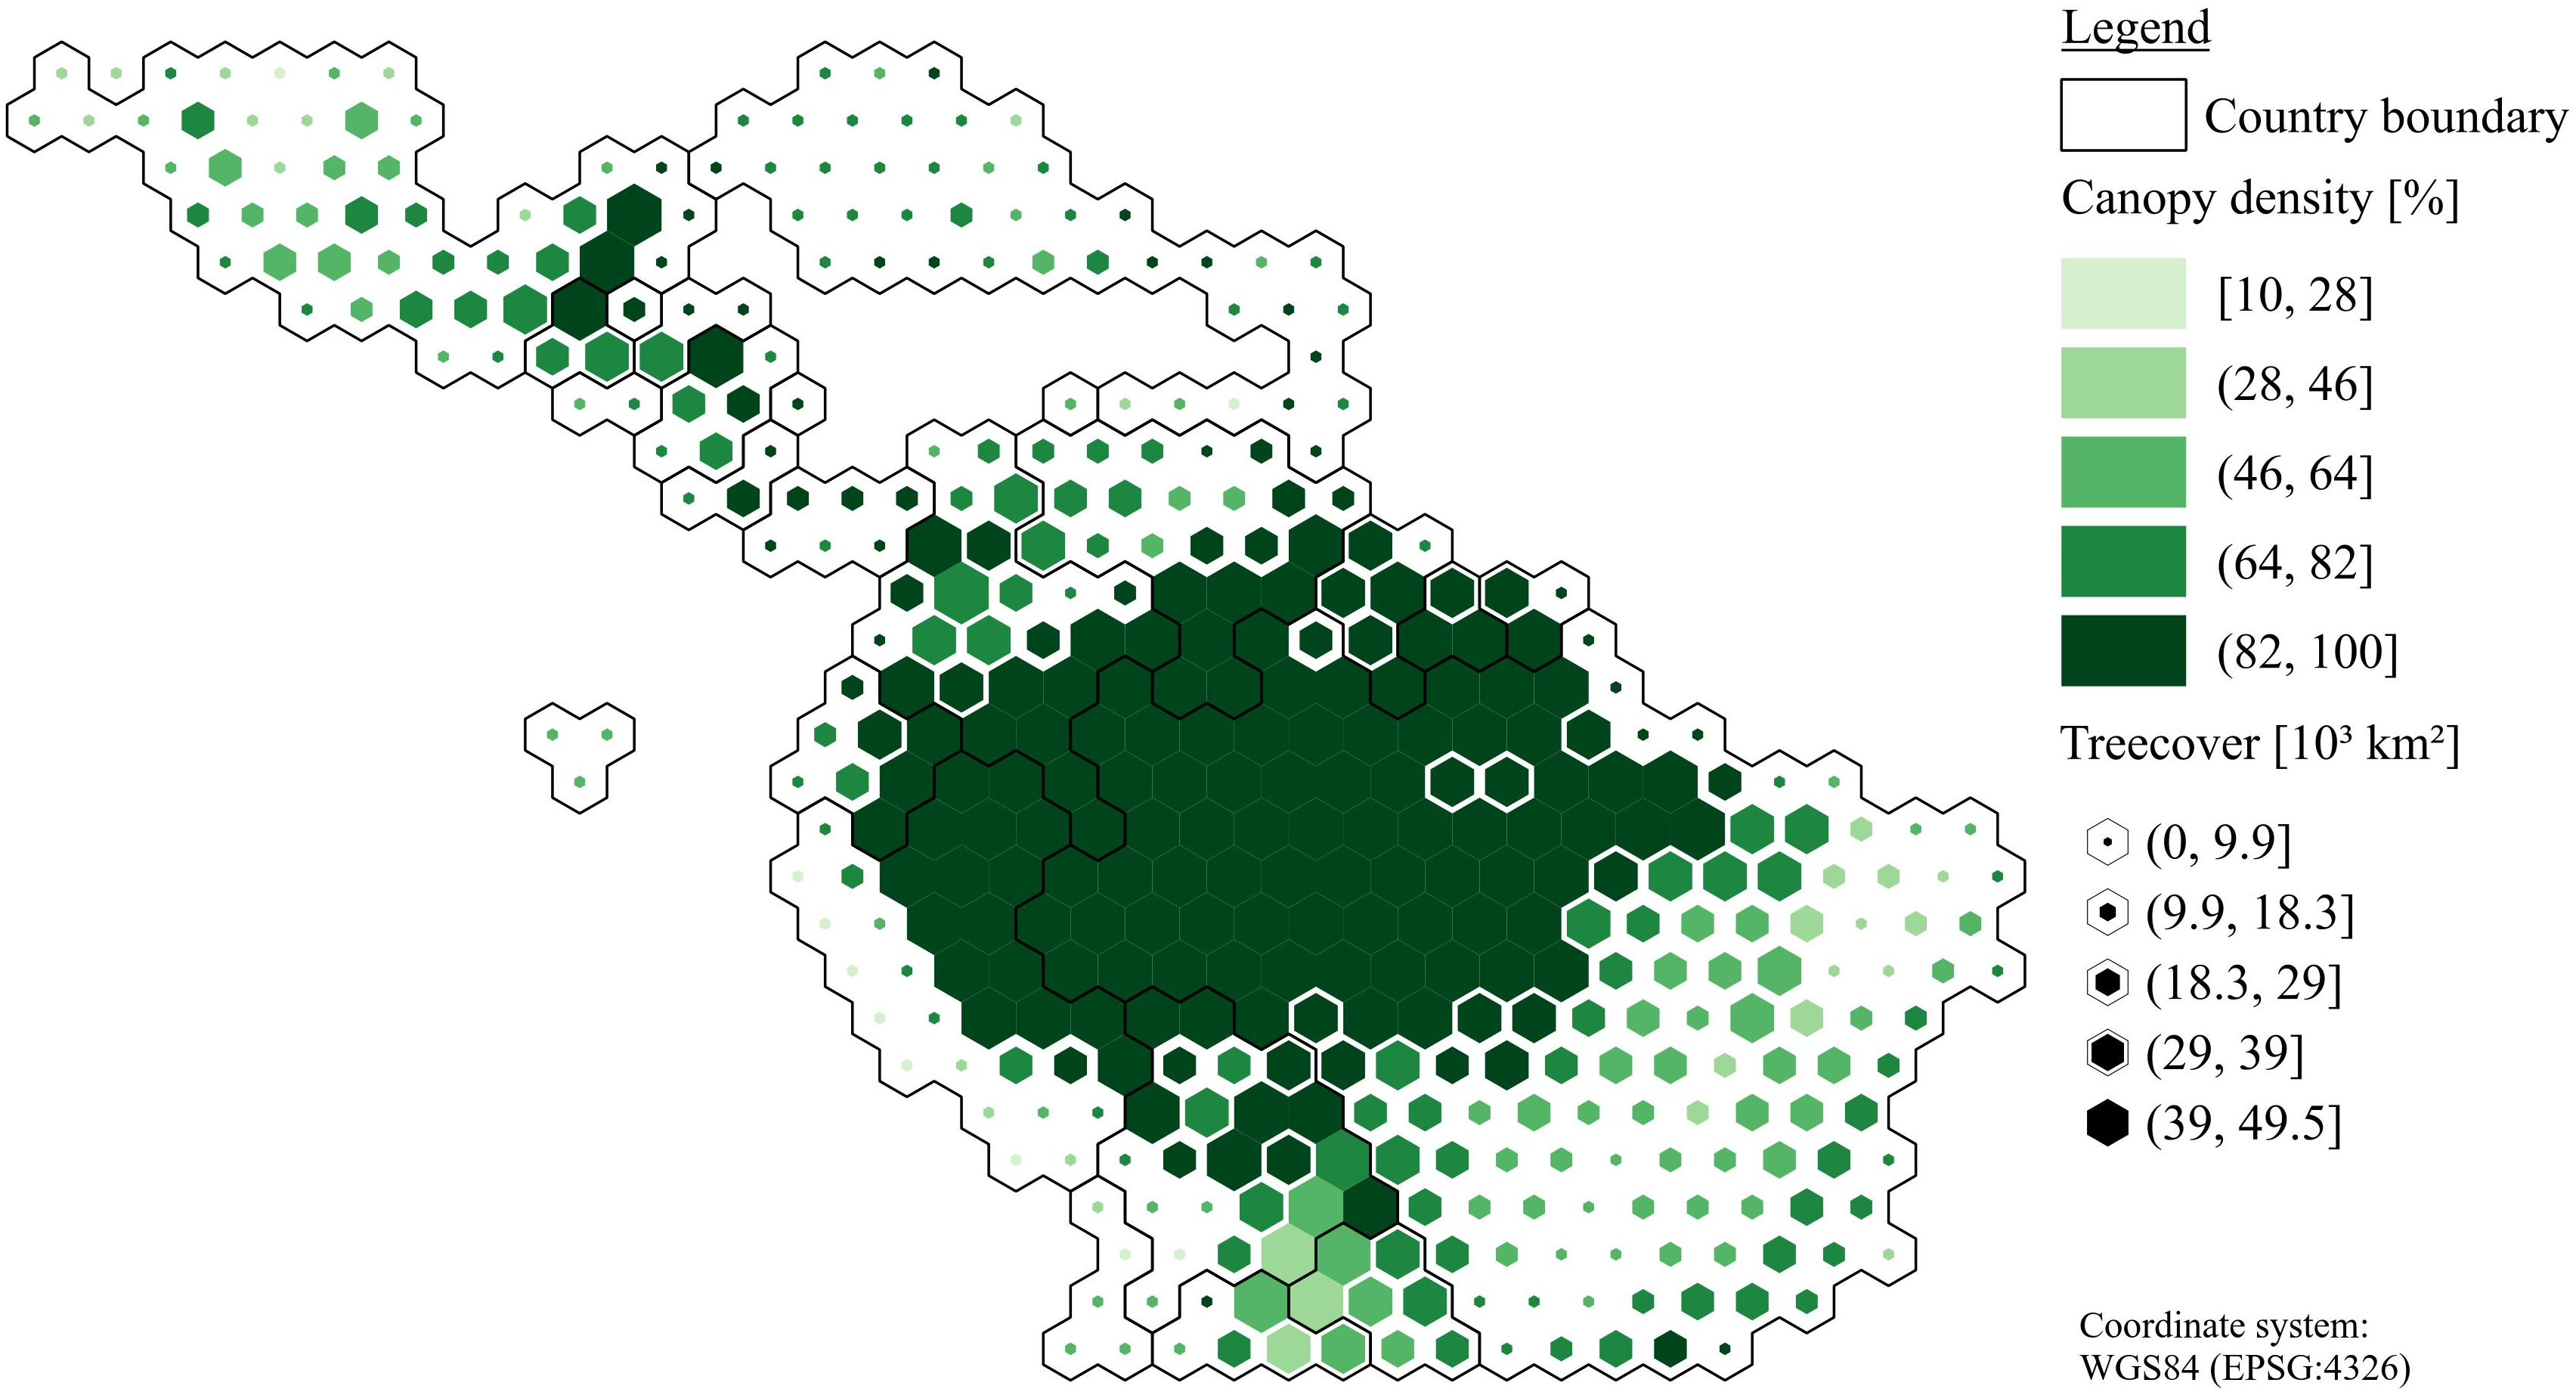
\includegraphics[scale=1]{img/americas_treecover_frameless}
%				\caption[Ecosystem service values]{}
%				\label{fig:americascover}
%			\end{figure}
%			\begin{figure}[ht]
%				\centering
%				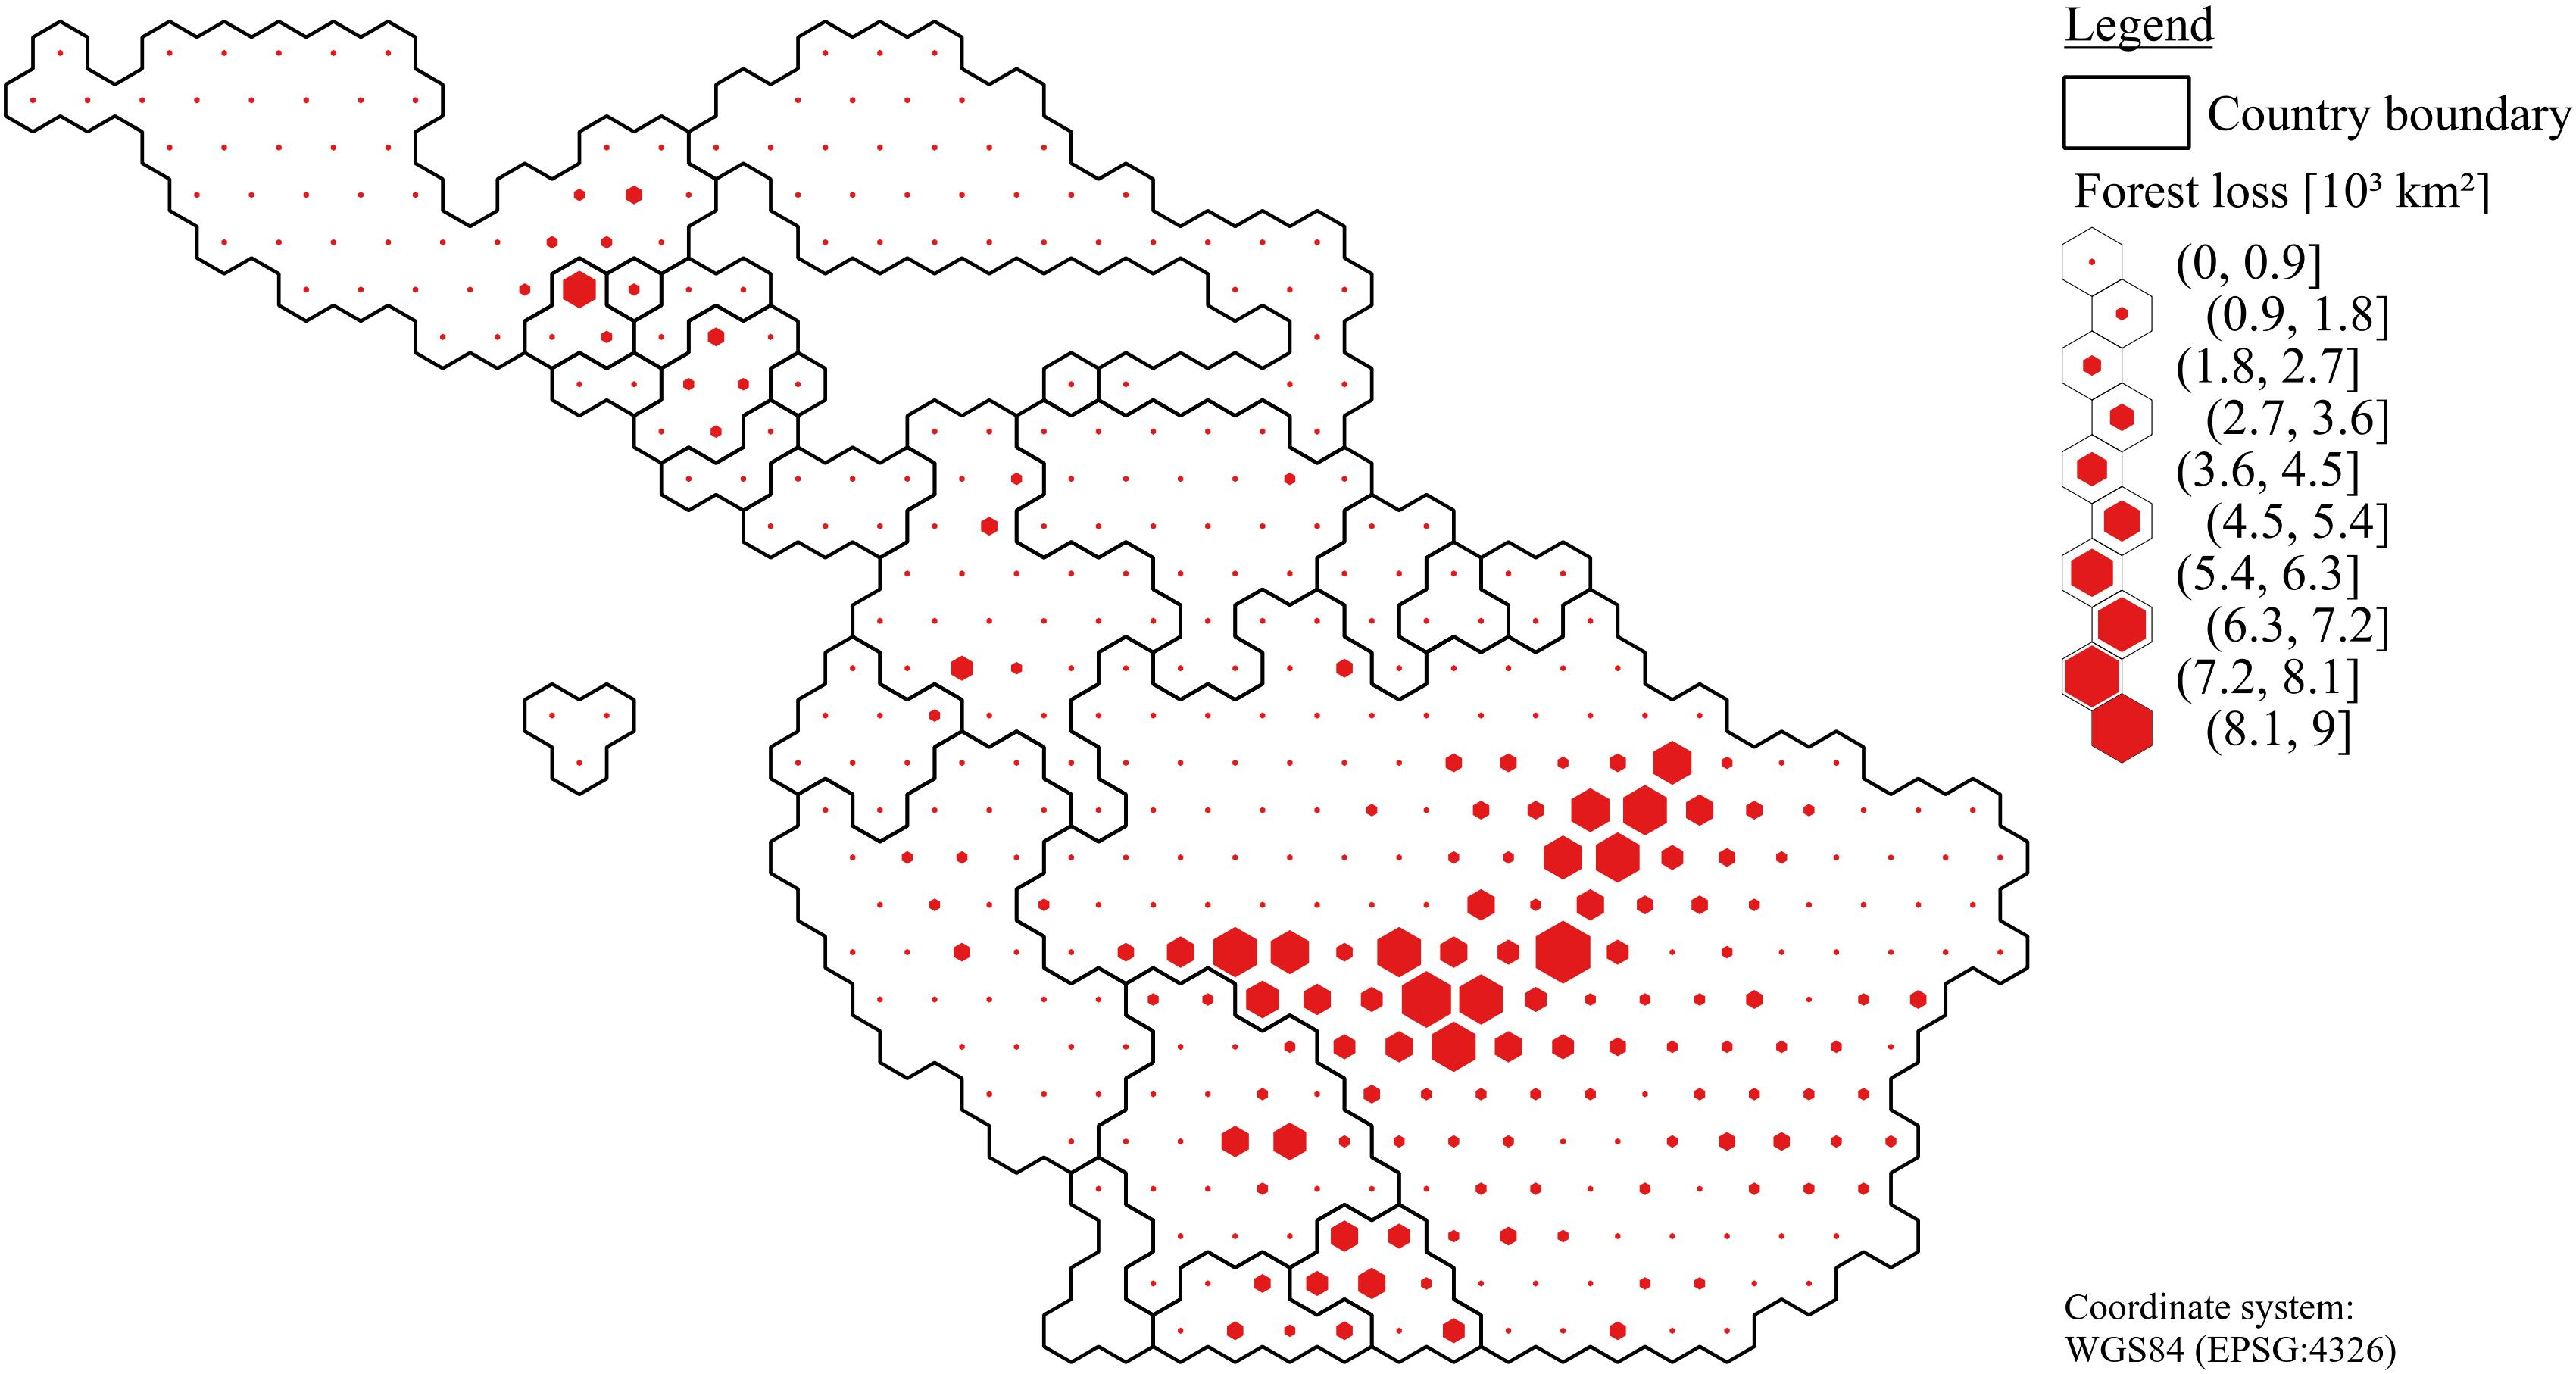
\includegraphics[scale=1]{img/americas_loss_frameless}
%				\caption[Ecosystem service values]{}
%				\label{fig:americasloss}
%			\end{figure}
%			\begin{figure}[ht]
%				\centering
%				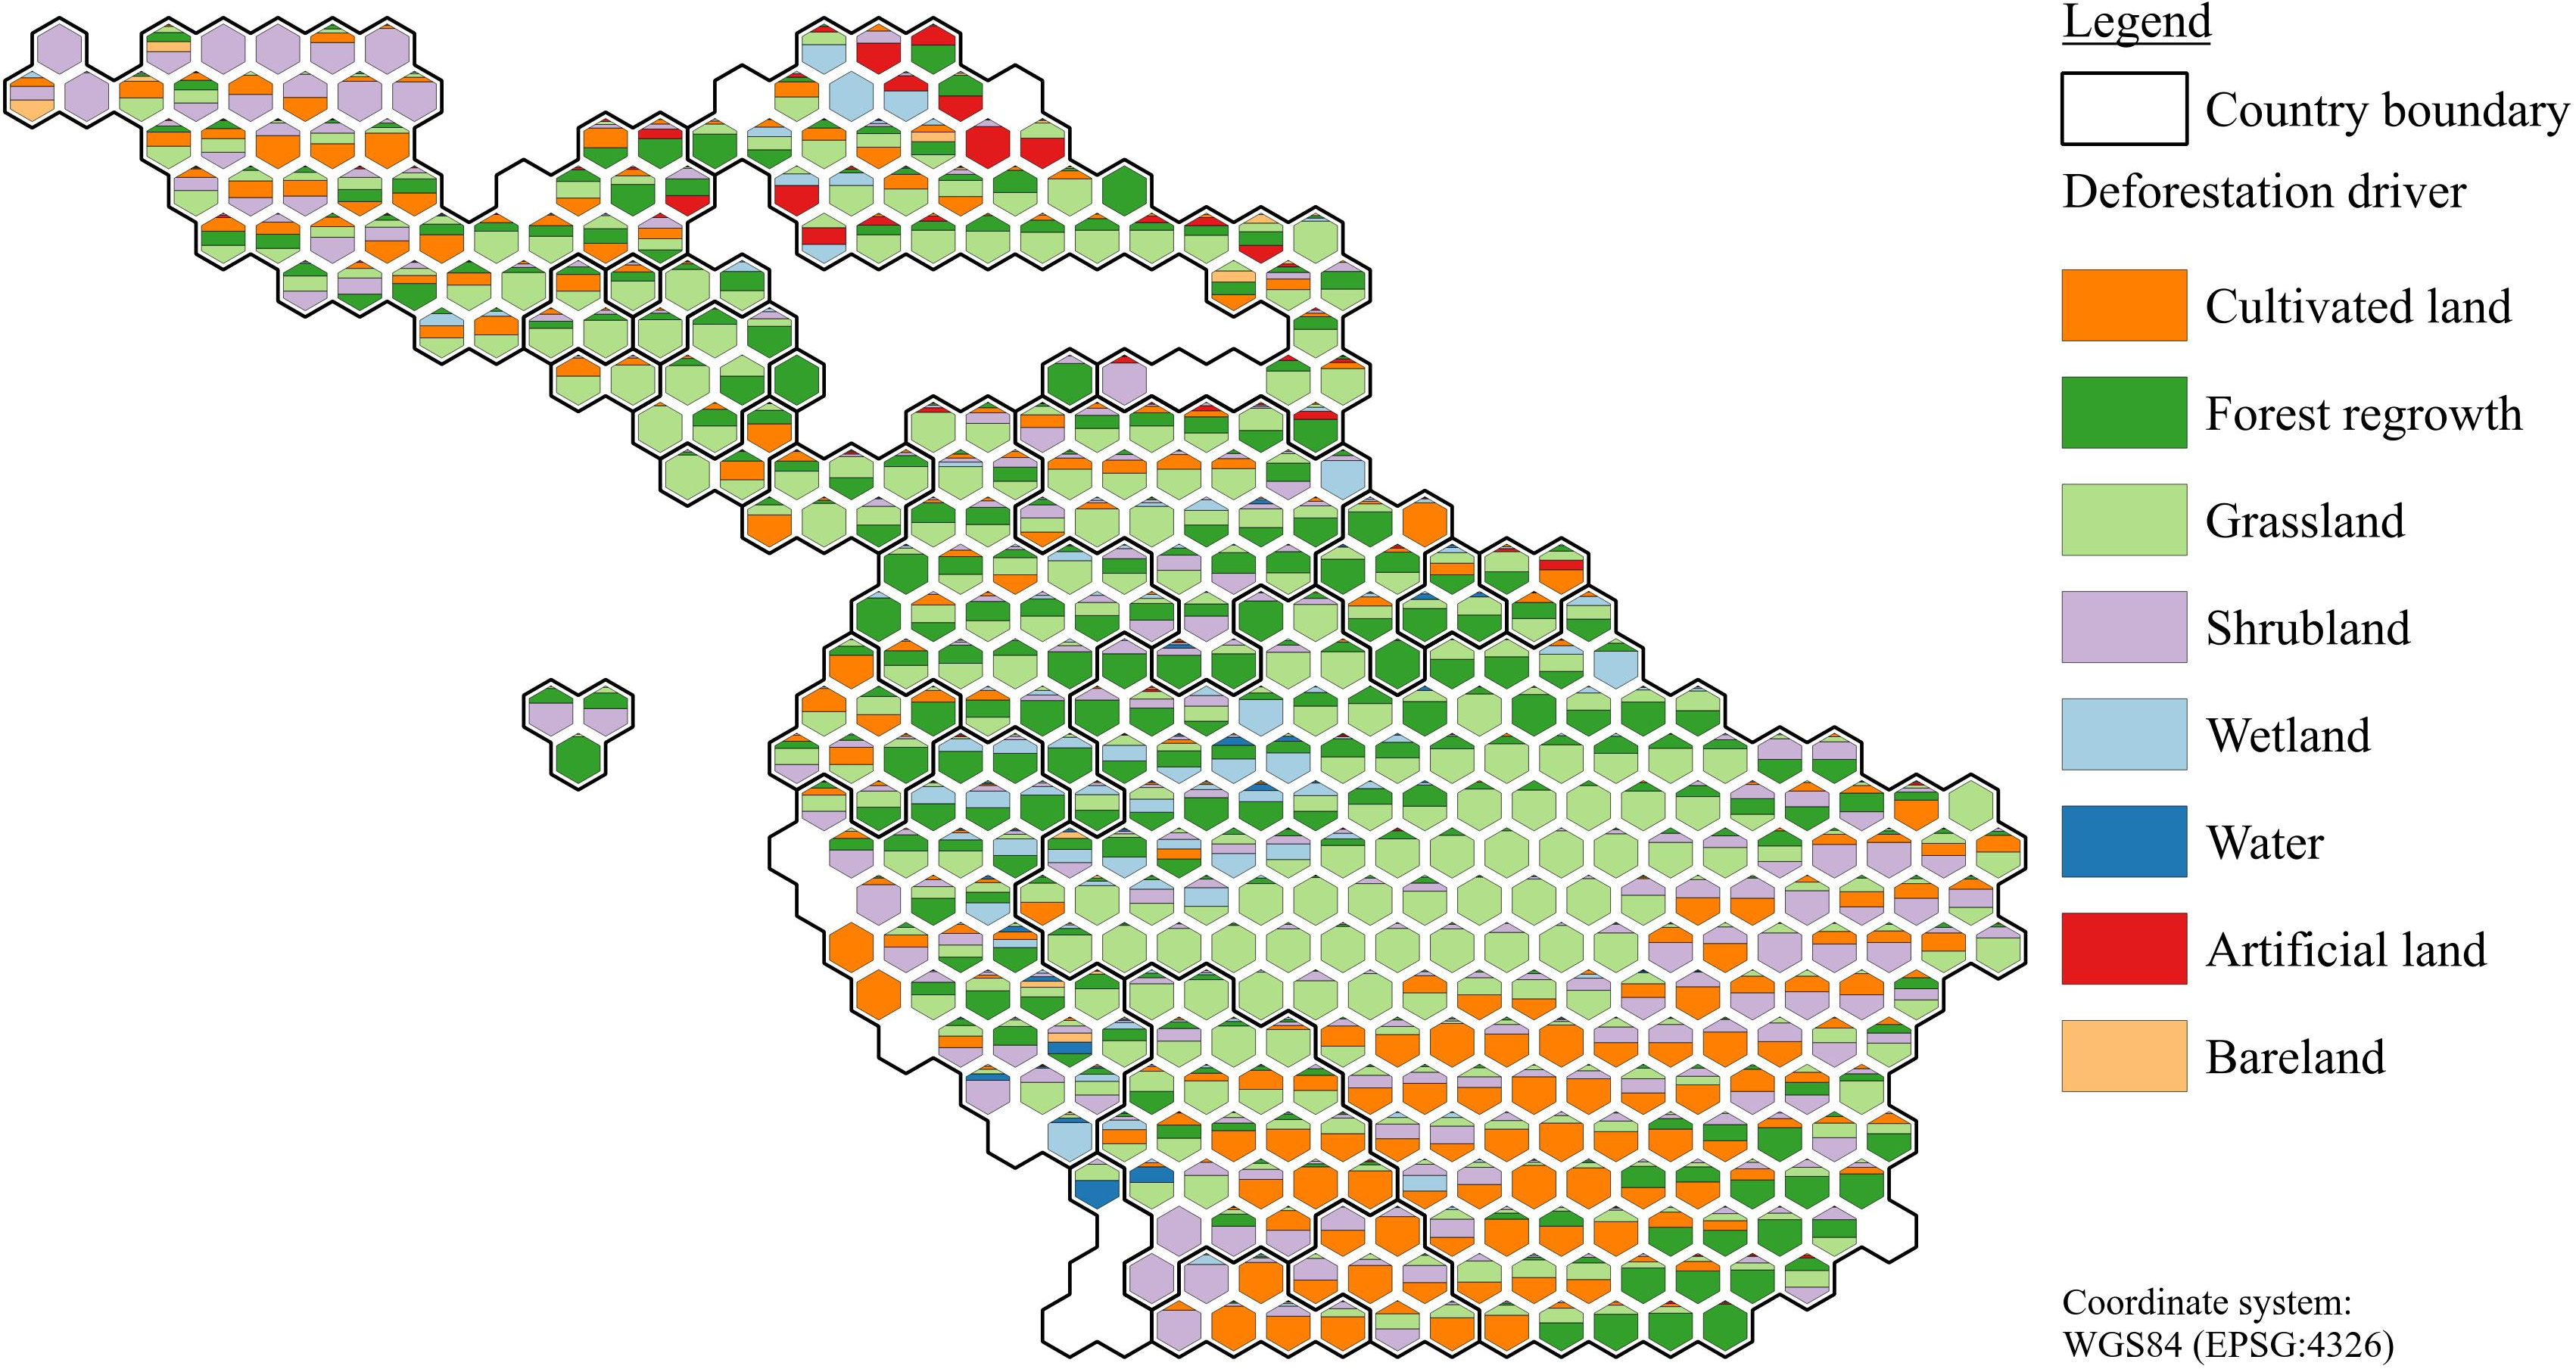
\includegraphics[scale=1]{img/americas_driver_frameless}
%				\caption[Ecosystem service values]{}
%				\label{fig:americasdriver}
%			\end{figure}

% ASIA
%			\begin{figure}[ht]
%				\centering
%				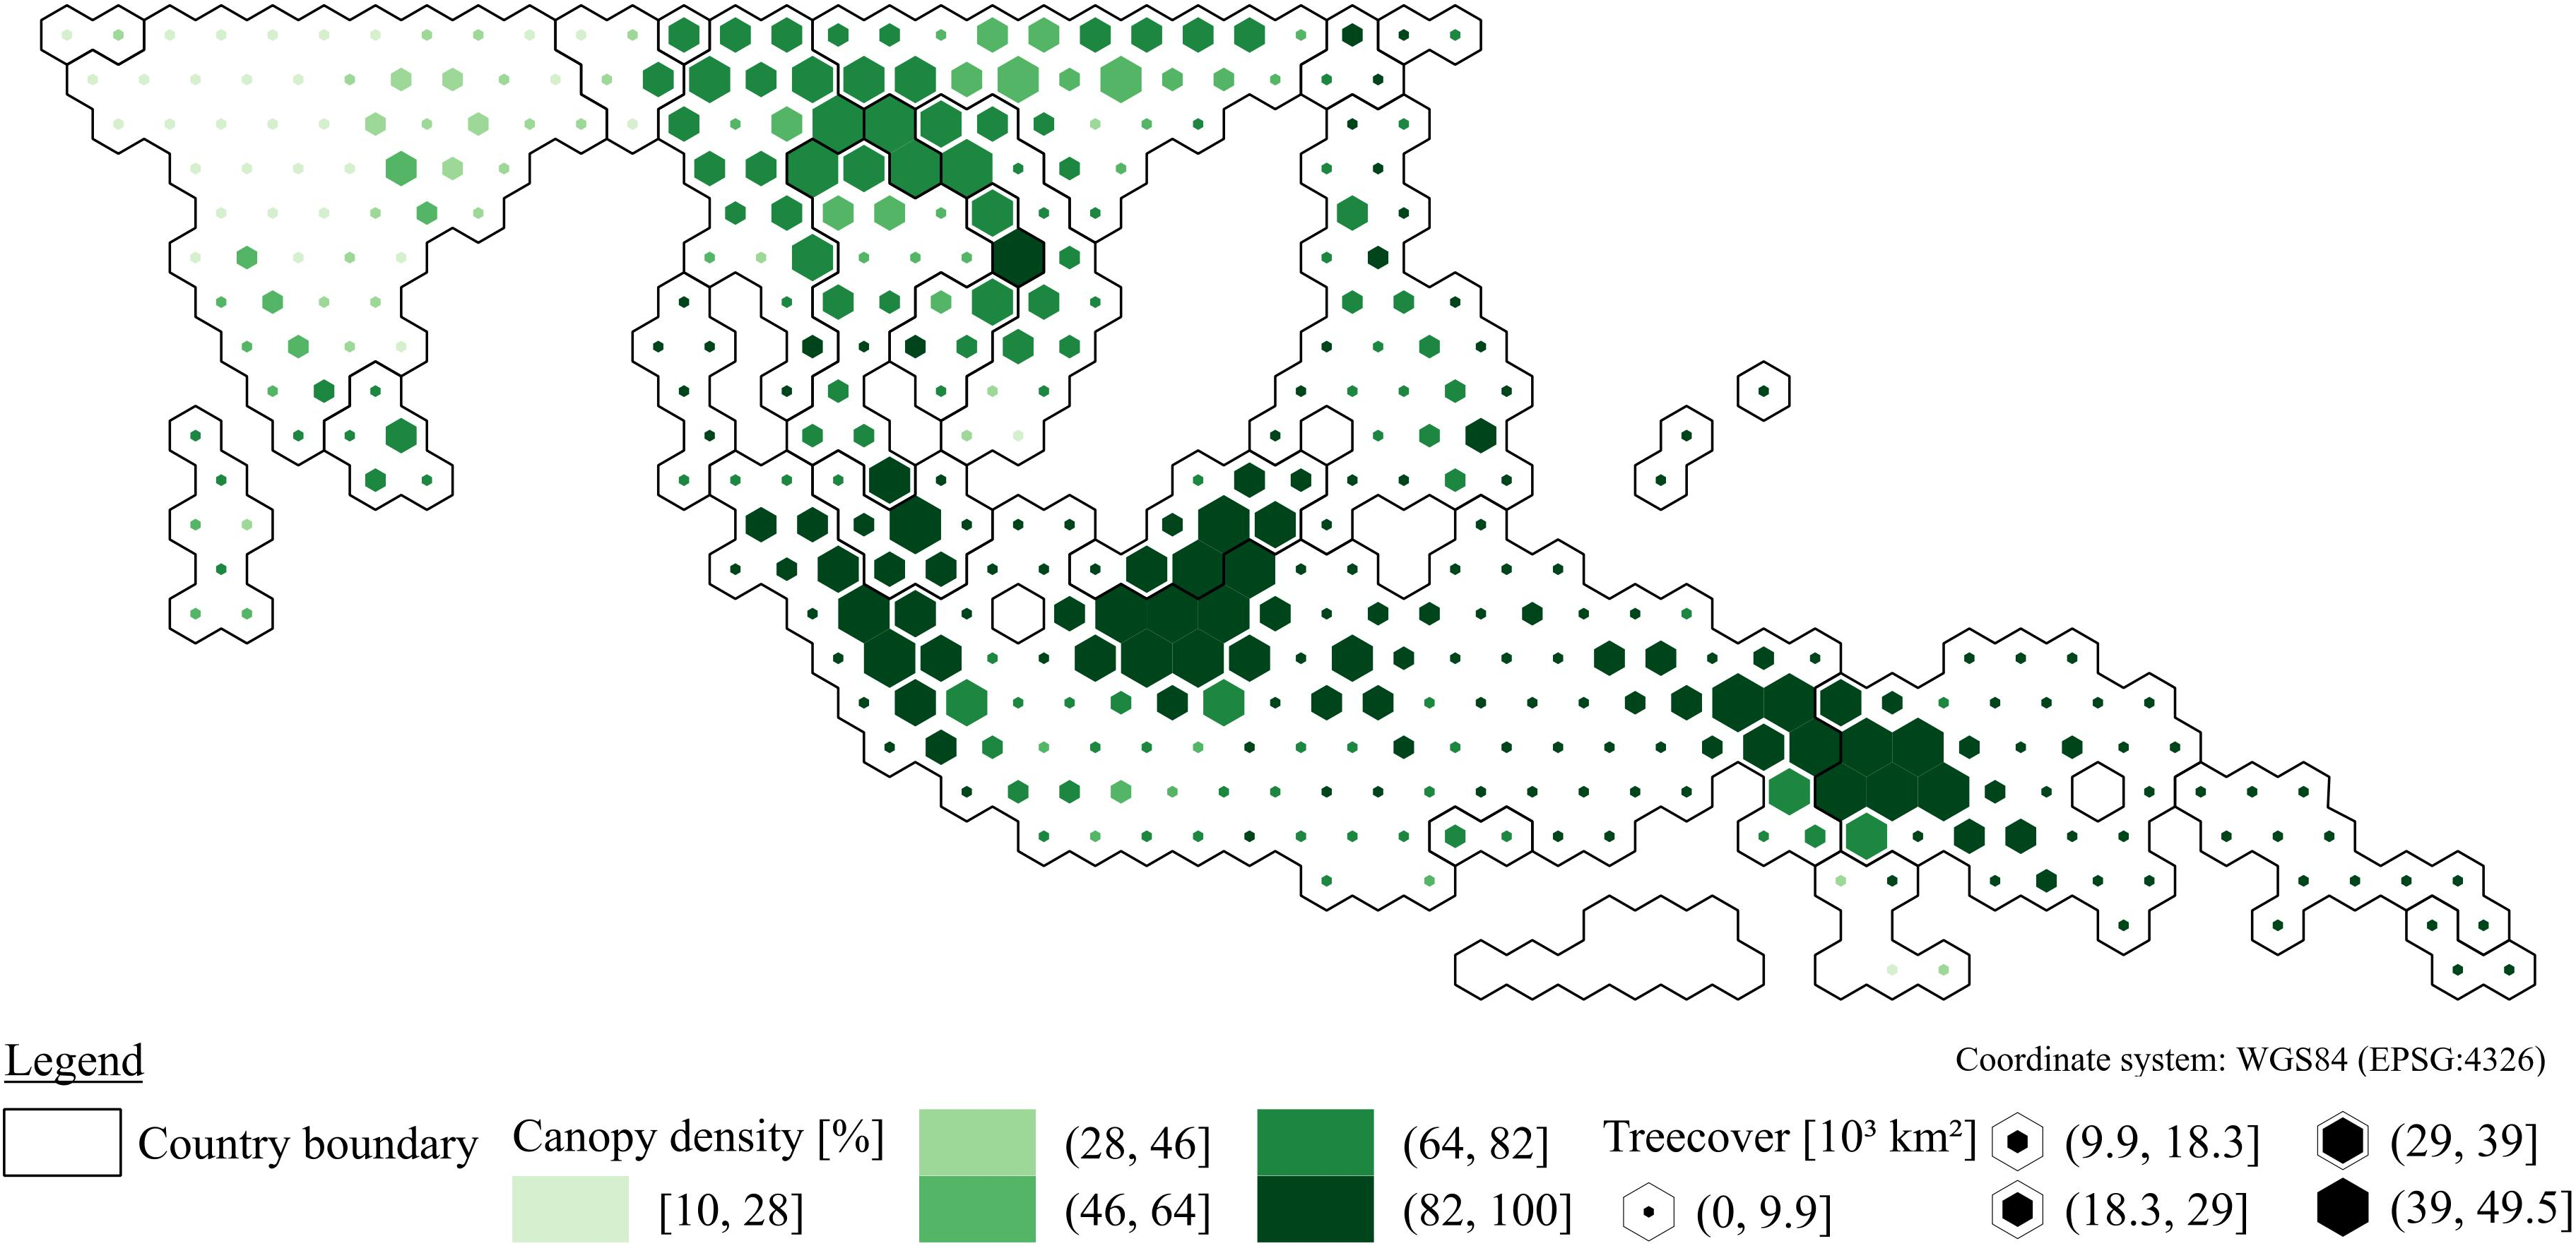
\includegraphics[scale=1]{img/asia_treecover_frameless}
%				\caption[Ecosystem service values]{}
%				\label{fig:asiacover}
%			\end{figure}
%			\begin{figure}[ht]
%				\centering
%				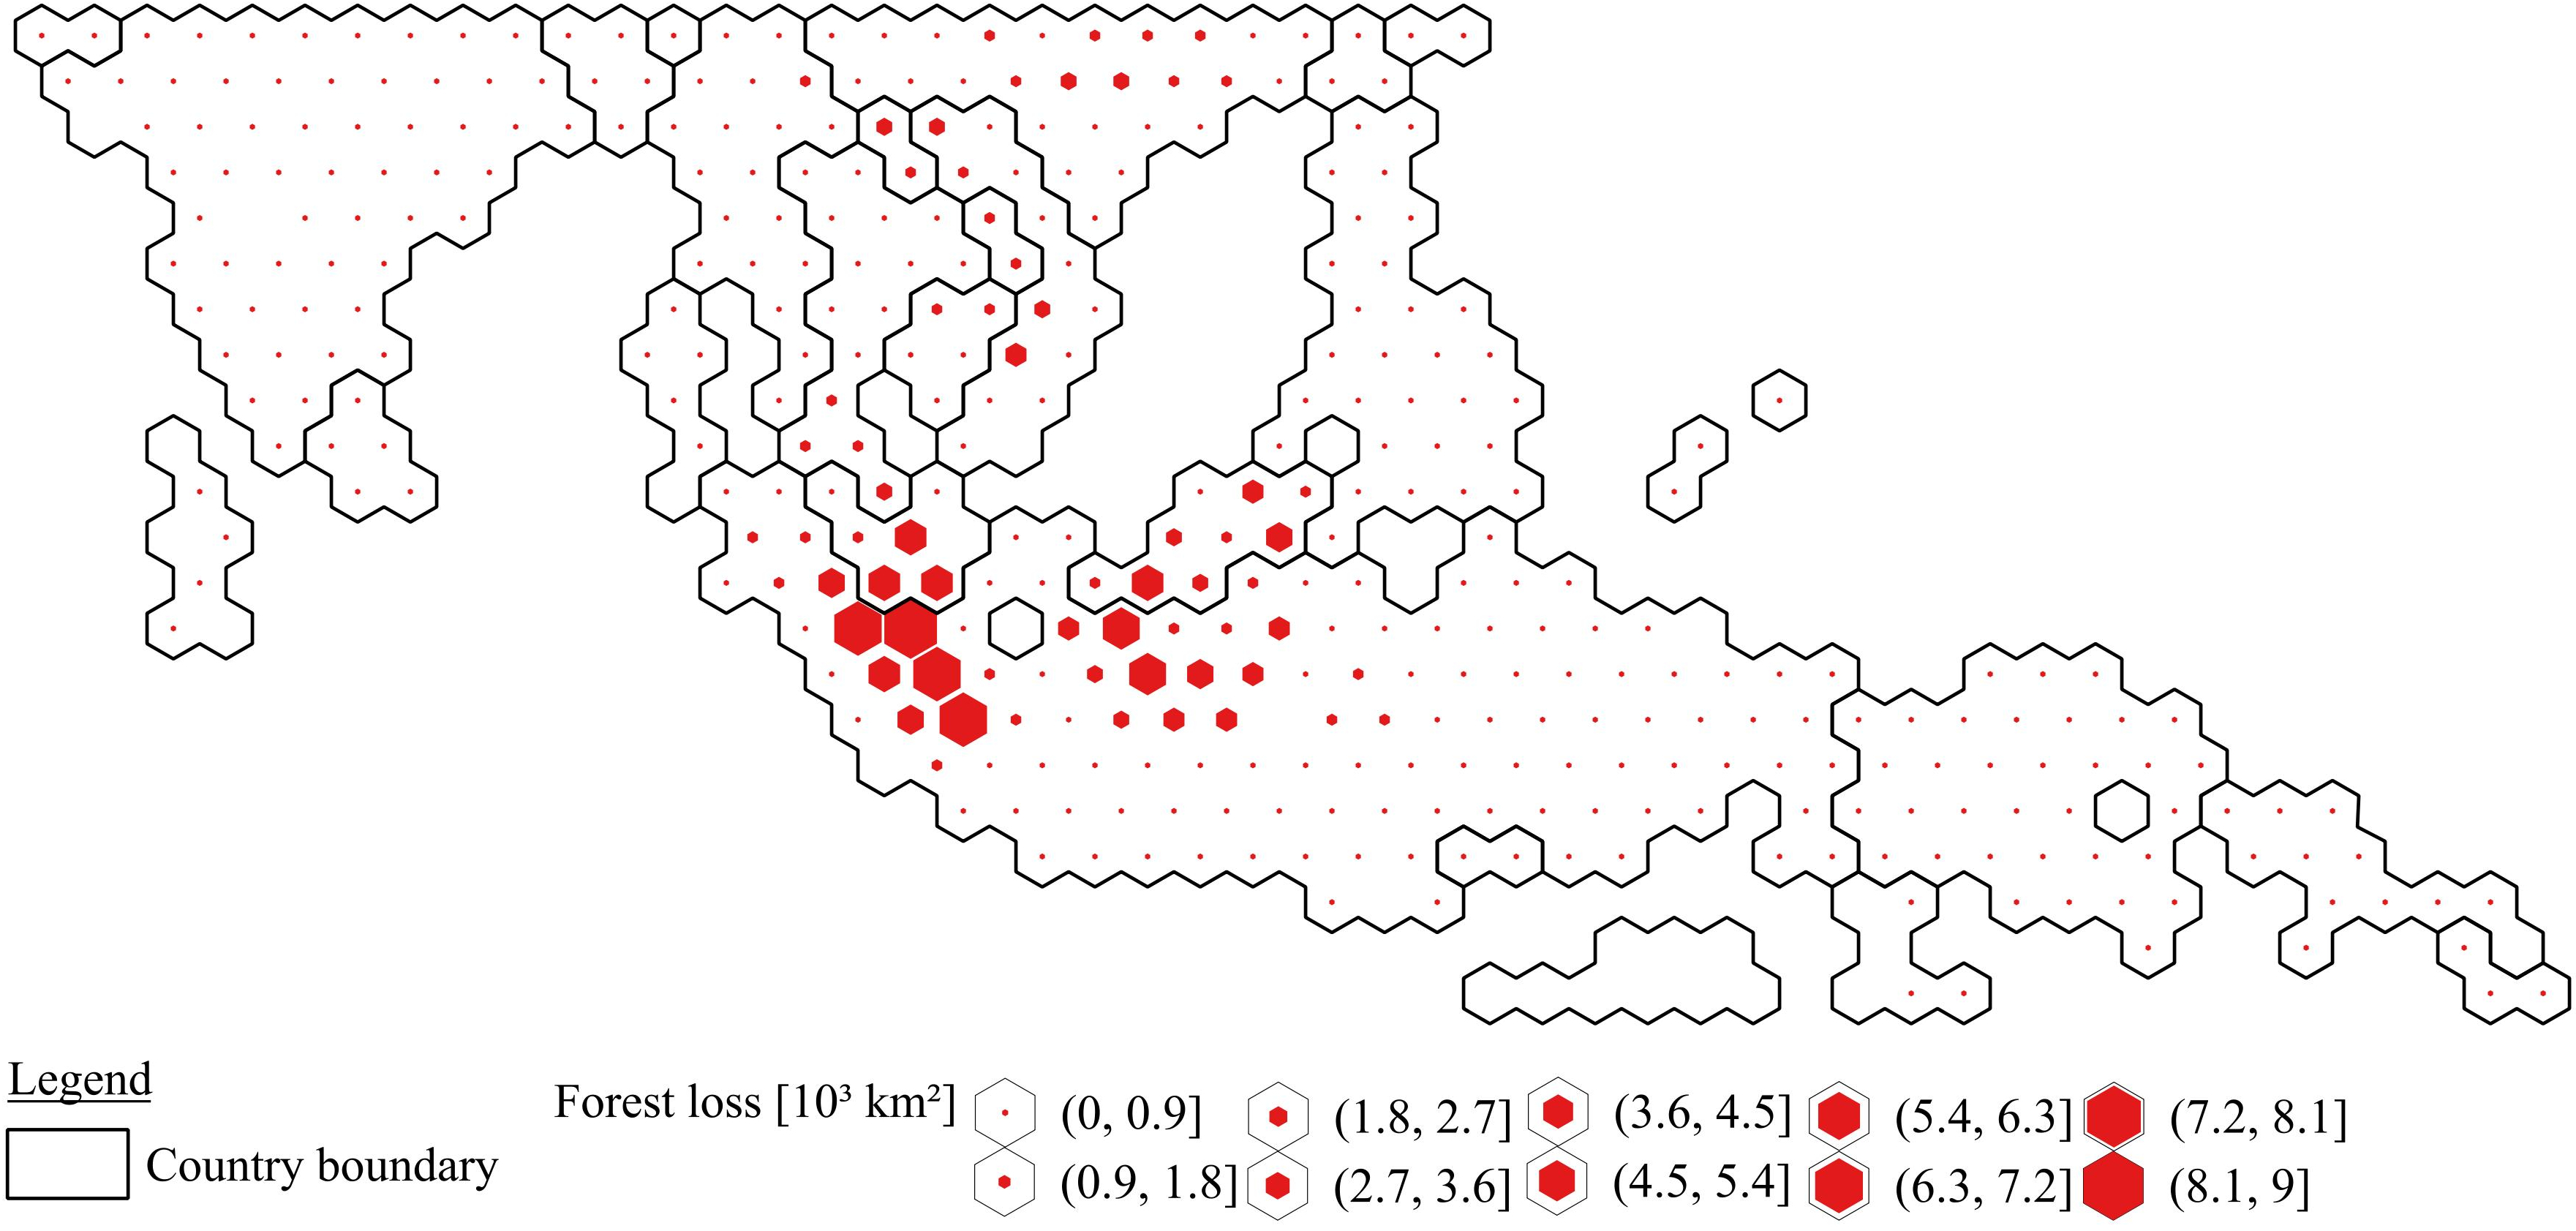
\includegraphics[scale=1]{img/asia_loss_frameless}
%				\caption[Ecosystem service values]{}
%				\label{fig:asialoss}
%			\end{figure}
%			\begin{figure}[ht]
%				\centering
%				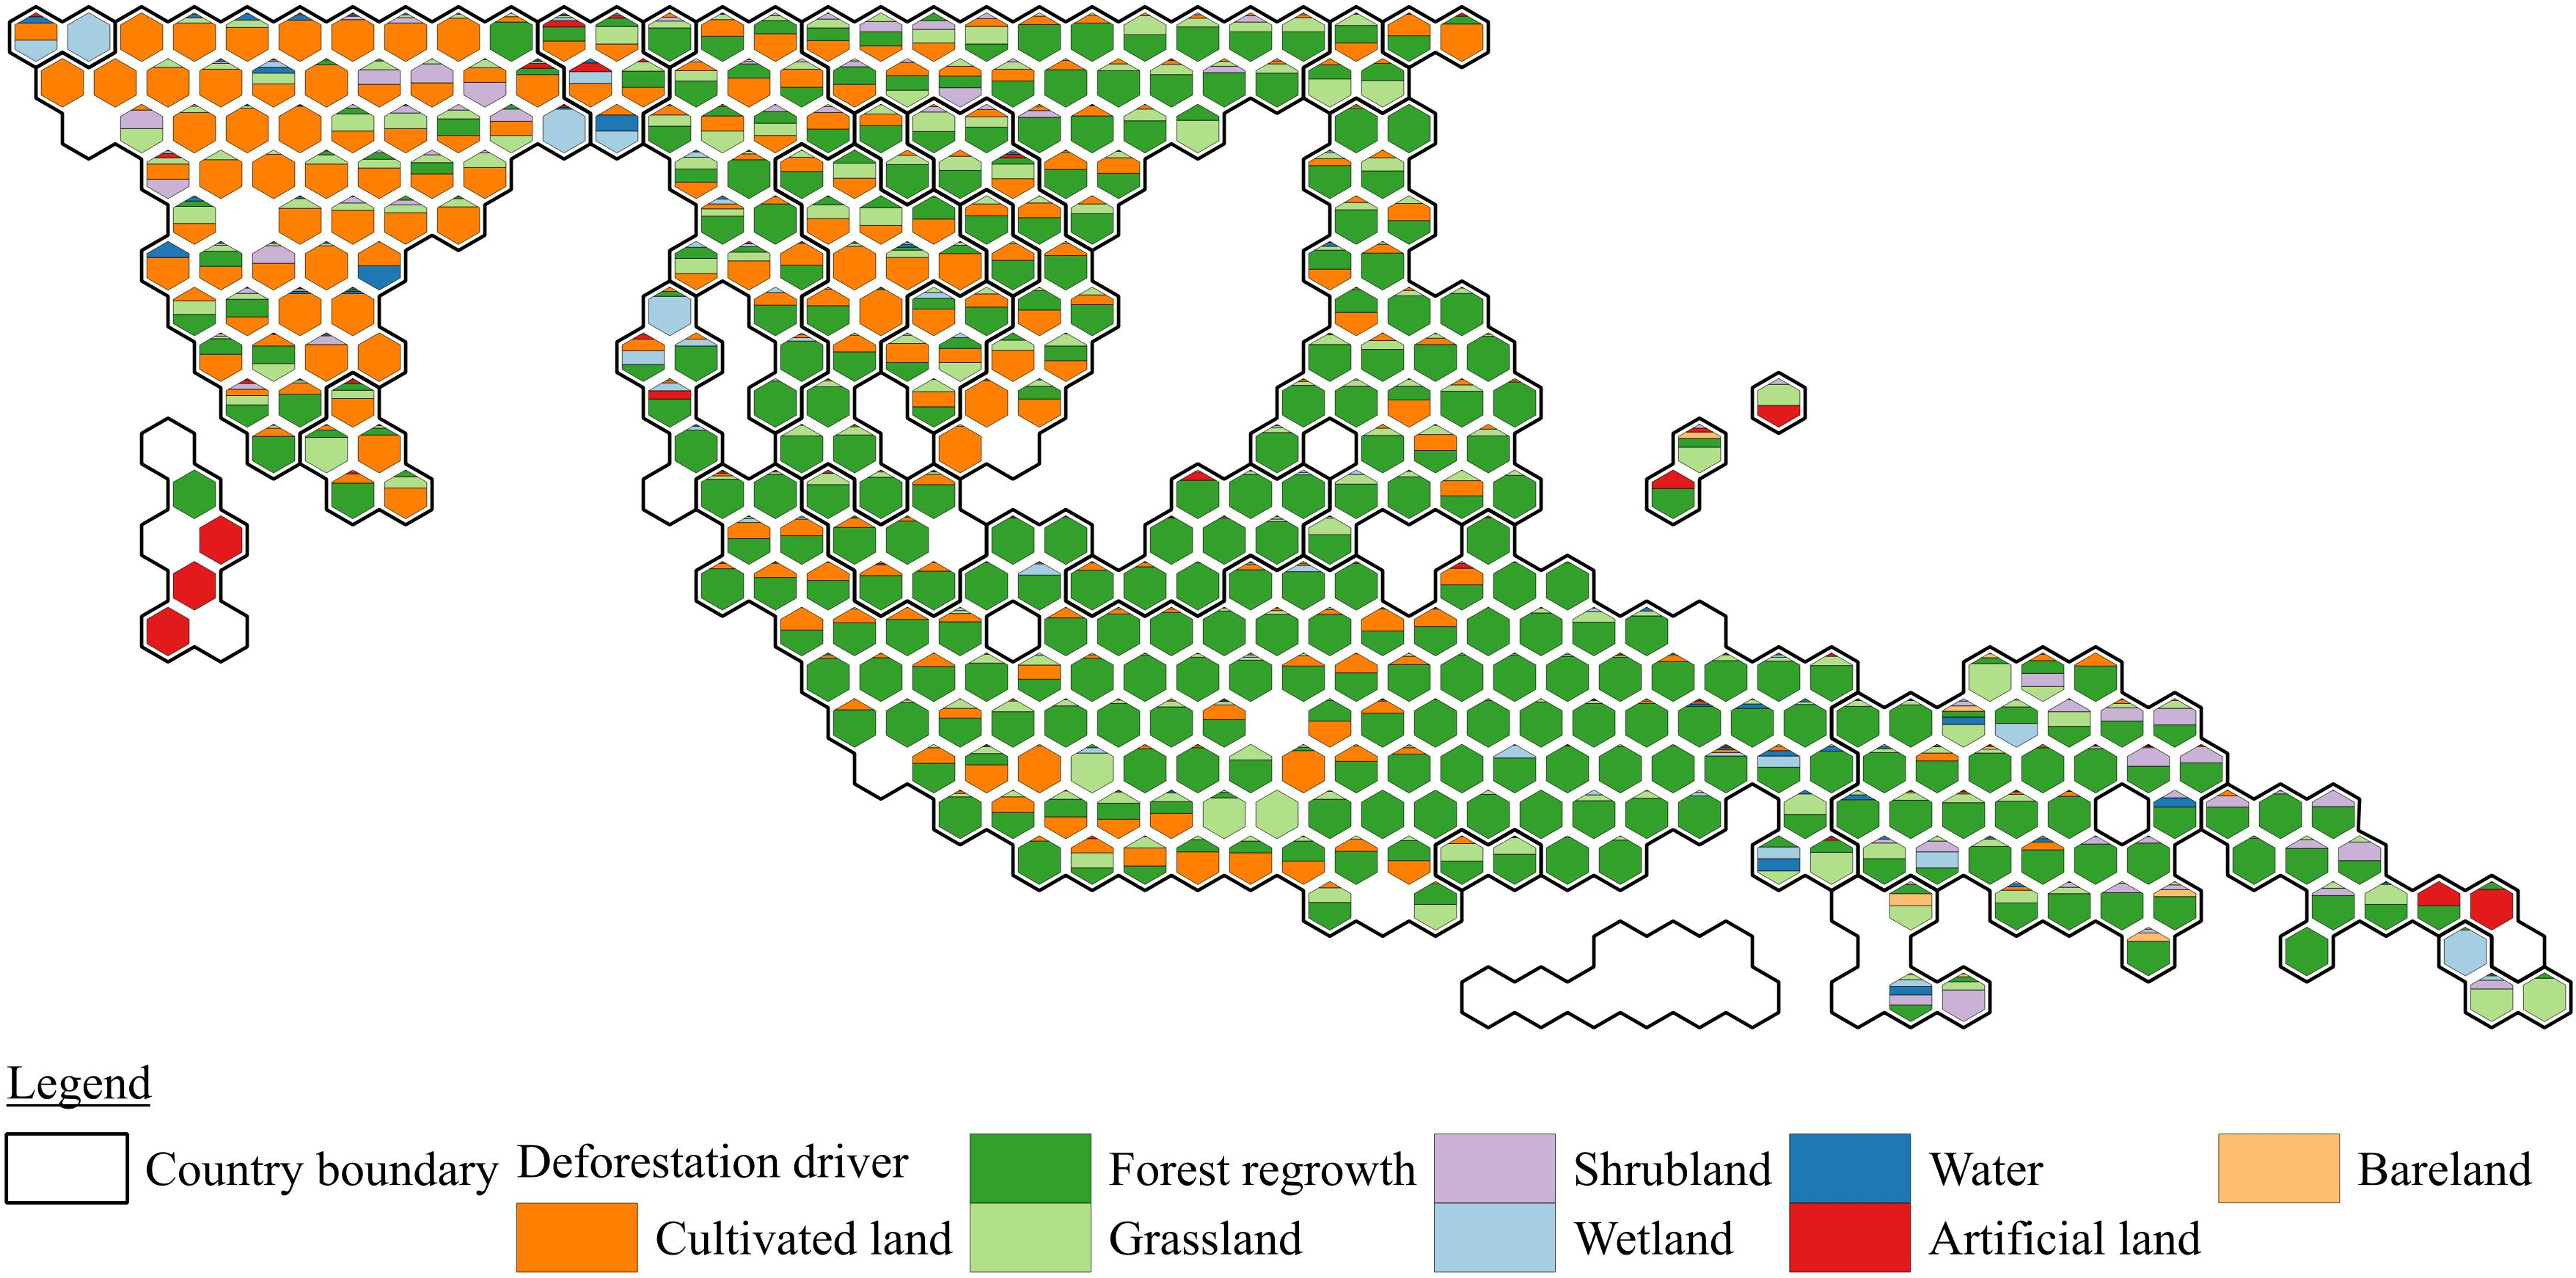
\includegraphics[scale=1]{img/asia_driver_frameless}
%				\caption[Ecosystem service values]{}
%				\label{fig:asiadriver}
%			\end{figure}

% AFRICA
%			\begin{figure}[ht]
%				\centering
%				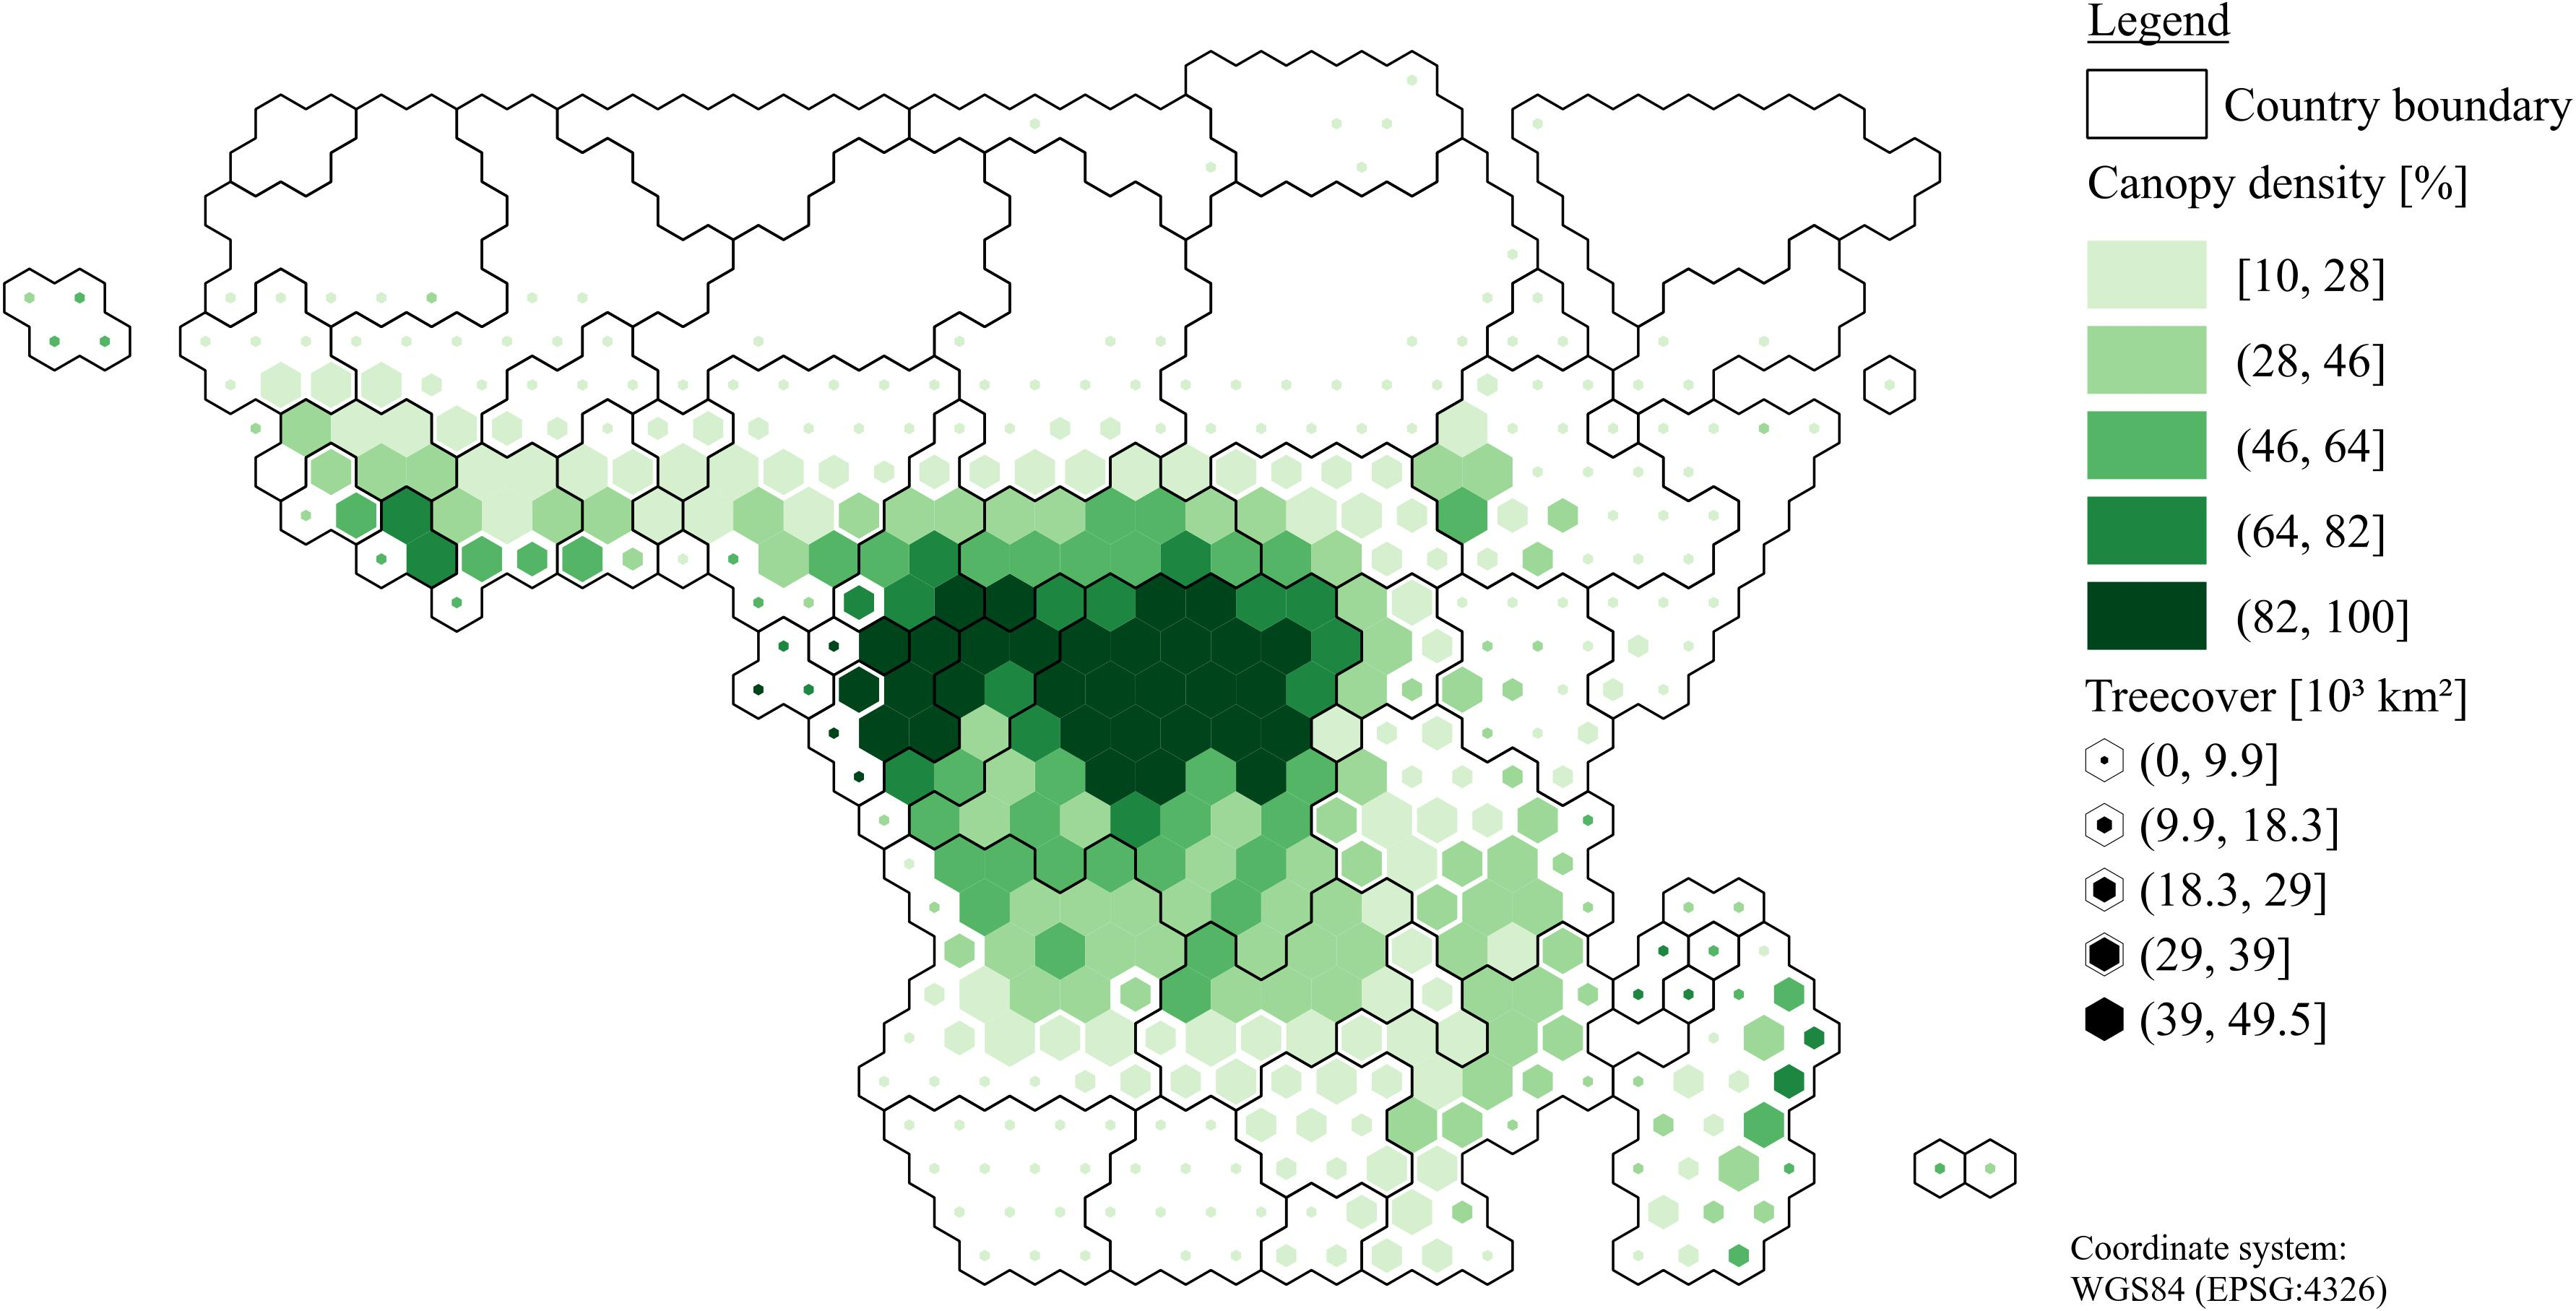
\includegraphics[scale=1]{img/africa_treecover_frameless}
%				\caption[Ecosystem service values]{}
%				\label{fig:africacover}
%			\end{figure}
%			\begin{figure}[ht]
%				\centering
%				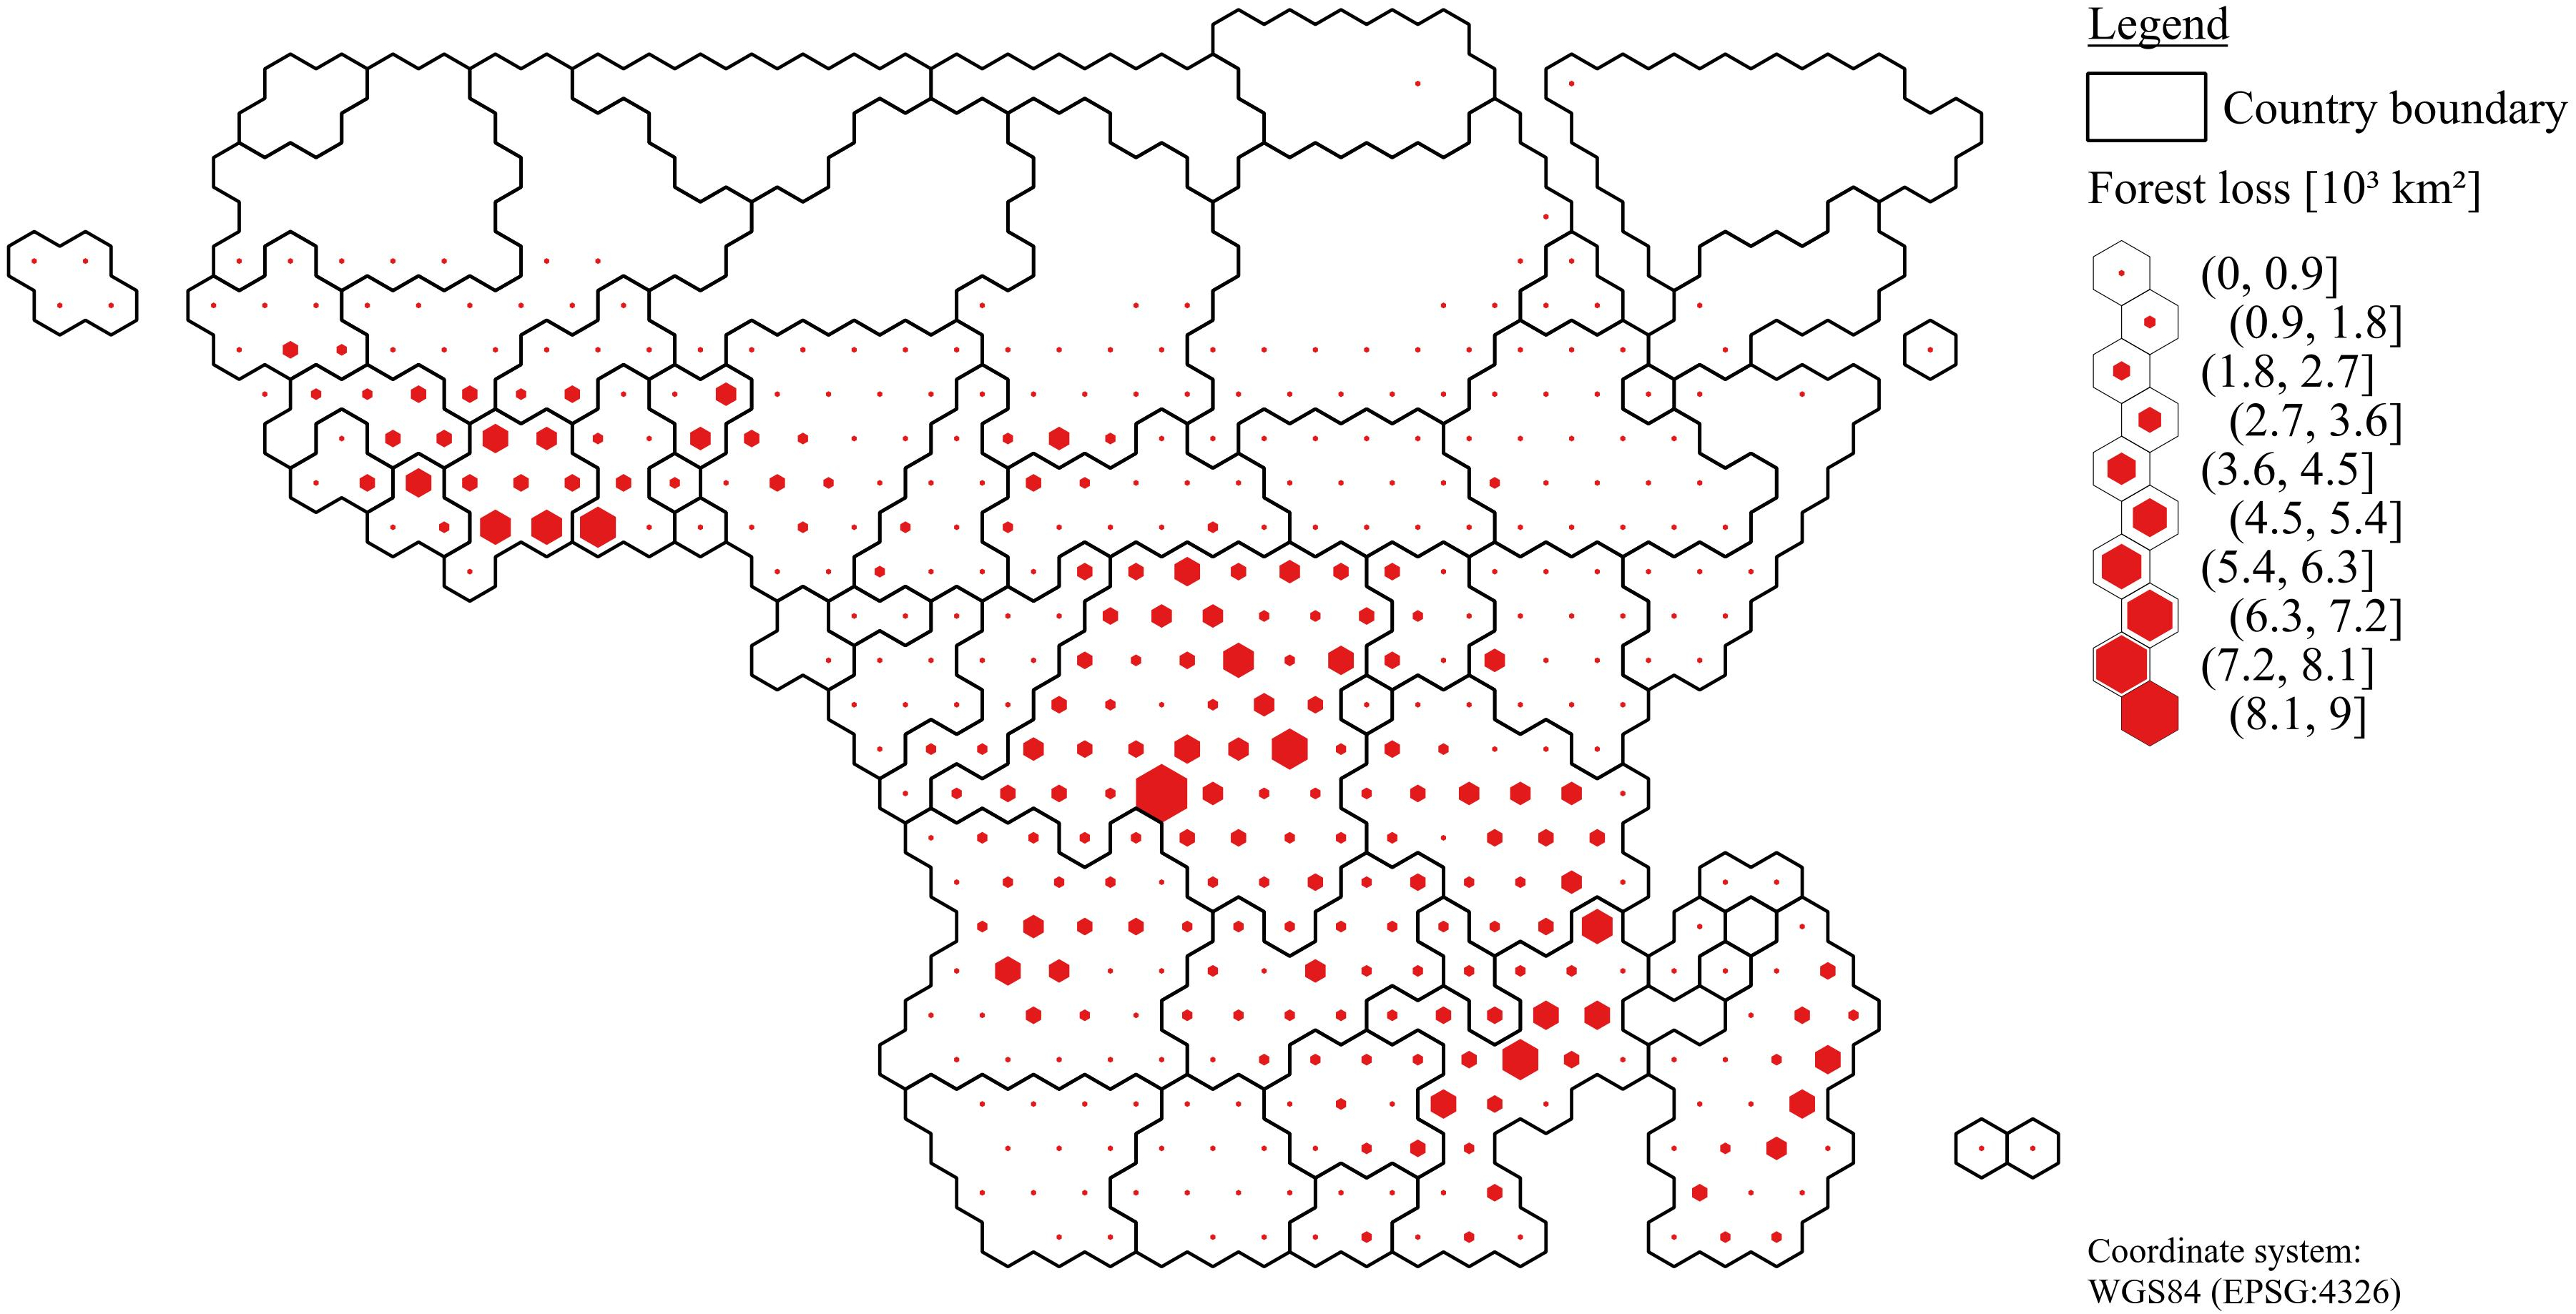
\includegraphics[scale=1]{img/africa_loss_frameless}
%				\caption[Ecosystem service values]{}
%				\label{fig:africaloss}
%			\end{figure}
%			\begin{figure}[ht]
%				\centering
%				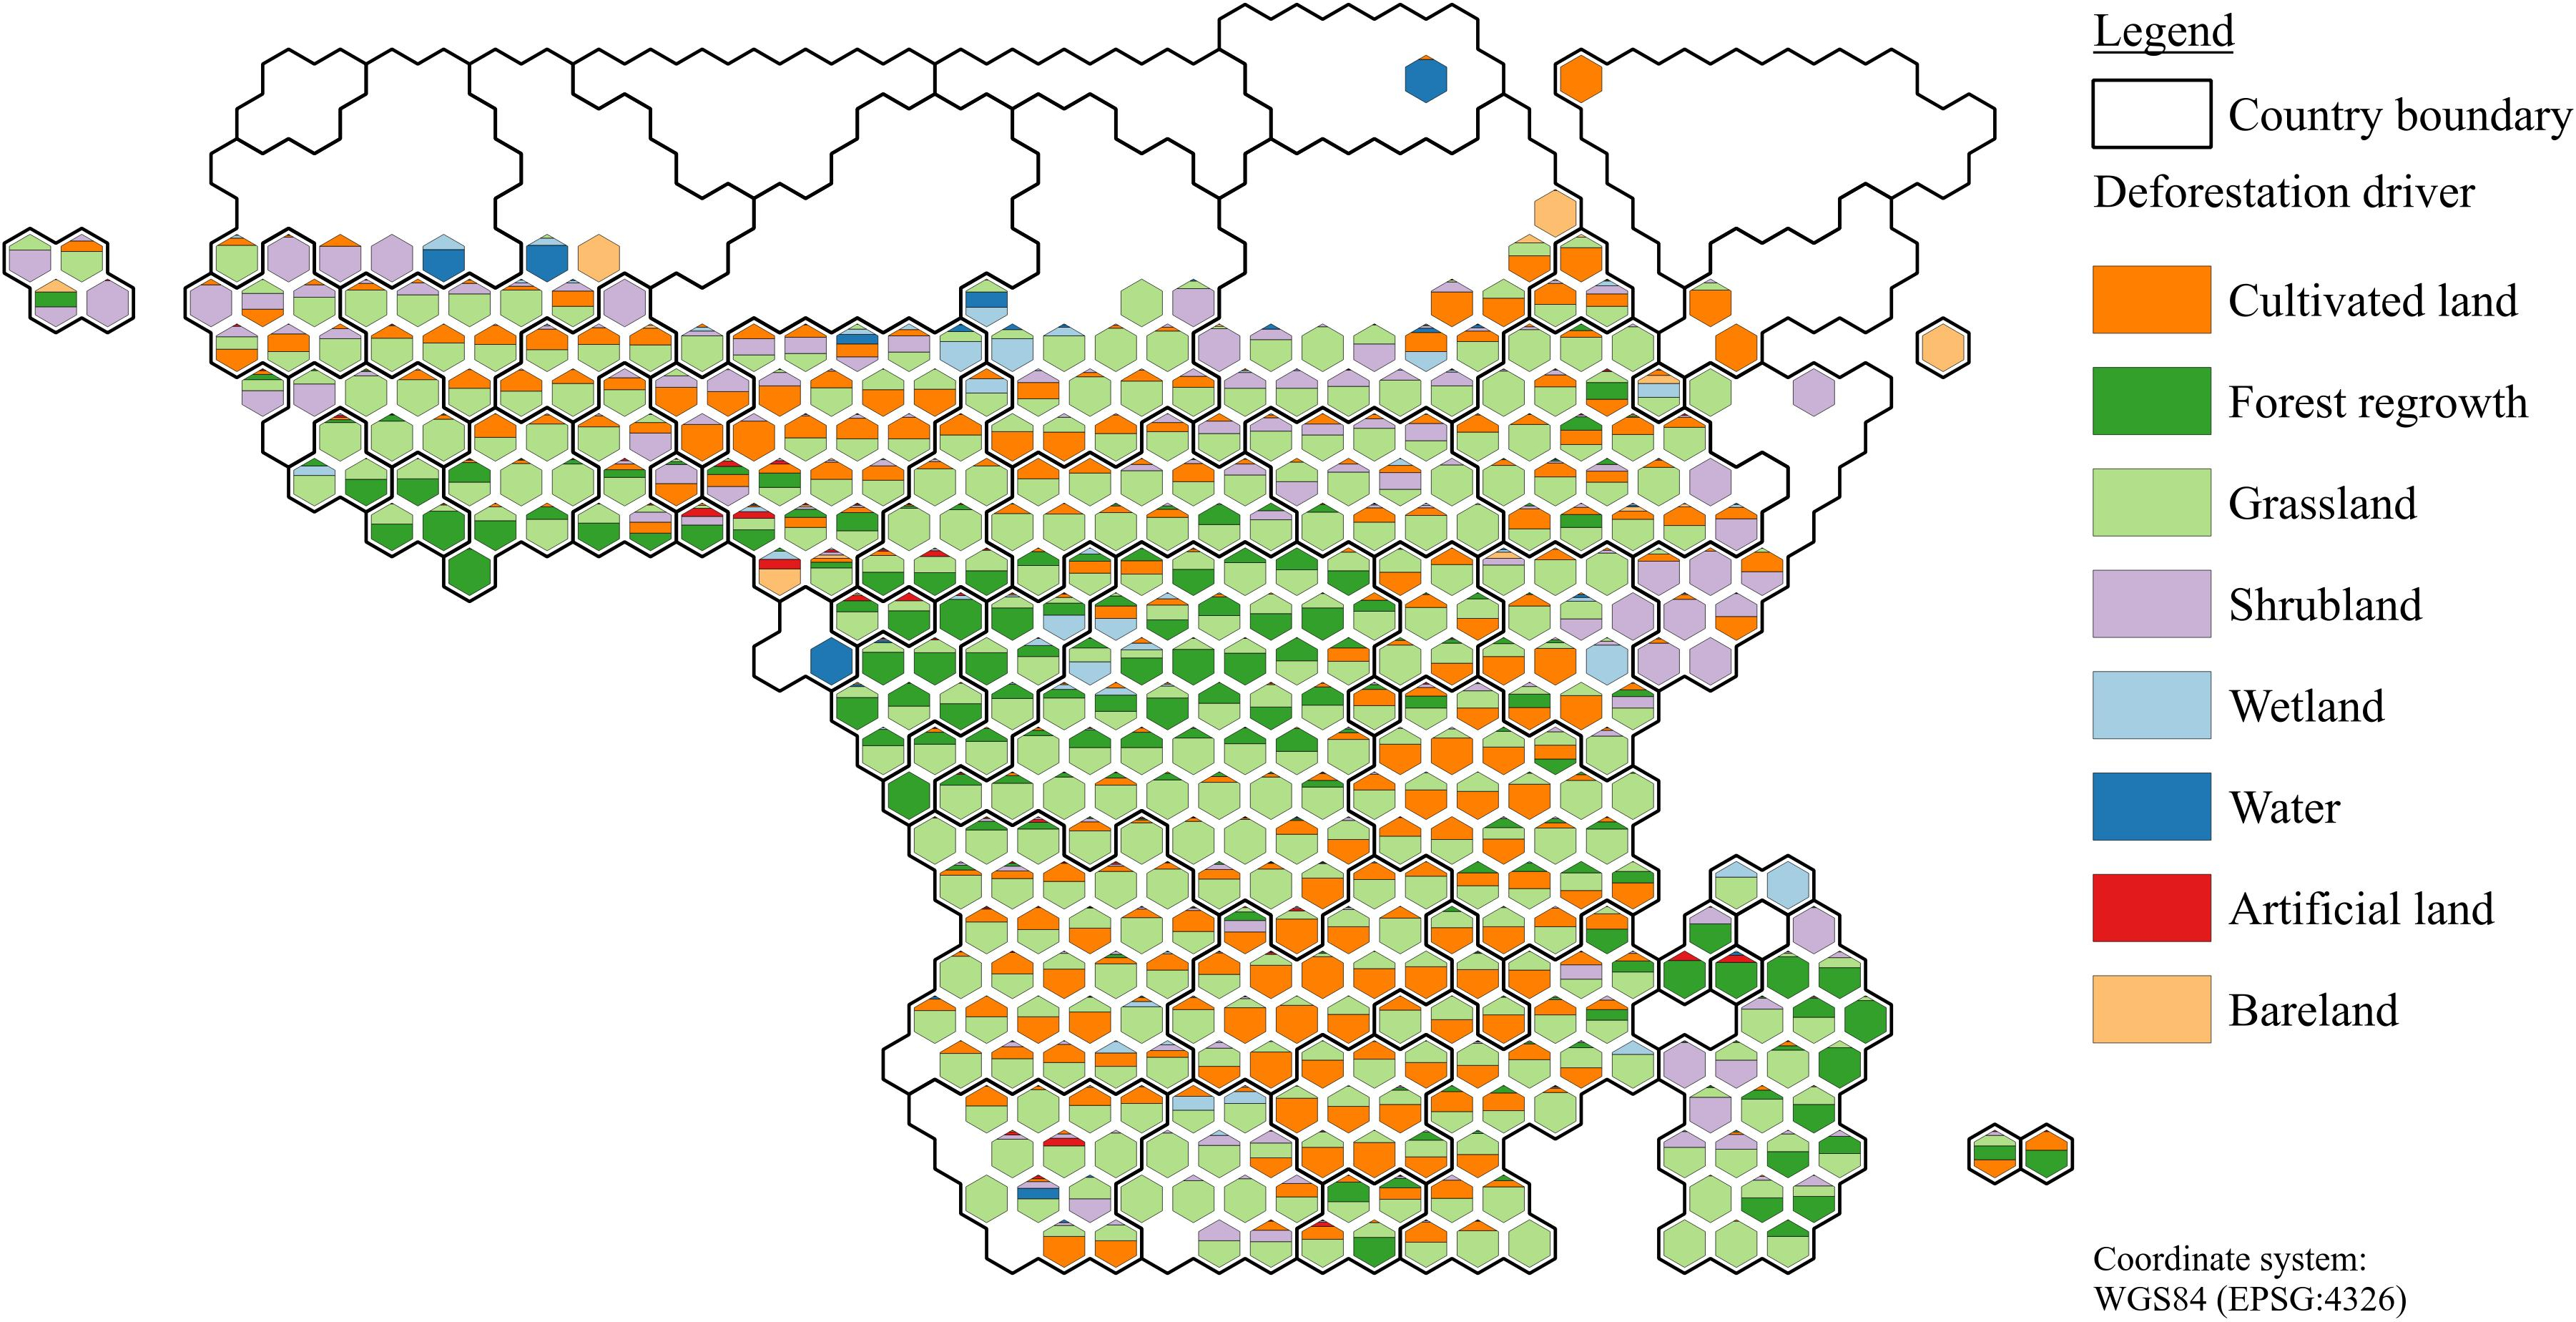
\includegraphics[scale=1]{img/africa_driver_frameless}
%				\caption[Ecosystem service values]{}
%				\label{fig:africadriver}
%			\end{figure}


% EMISSIONS
%		\begin{figure}[ht]
%			\centering
%			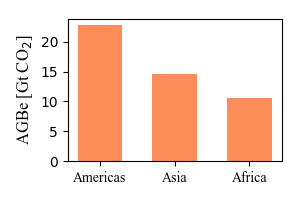
\includegraphics[scale=1]{img/agbe}
%			\caption[Ecosystem service values]{}
%			\label{fig:agbe}
%		\end{figure}
%		\begin{figure}[ht]
%			\centering
%			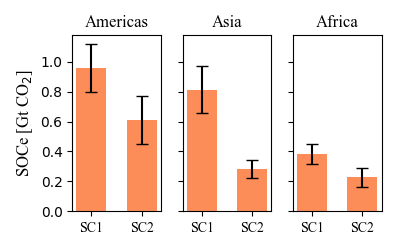
\includegraphics[scale=1]{img/soce}
%			\caption[Ecosystem service values]{}
%			\label{fig:soce}
%		\end{figure}
%
%		\begin{table}[ht]
%			\centering
%			\caption[Soil organic carbon emissions]{Soil organic carbon emissions}
%			\label{tab:soce_tab}
%			\begin{tabular}{lrrrrrrrrr}
%				\hline
%				\multirow{3}{*}{Region} & \multicolumn{3}{c}{SC1}& \multicolumn{3}{c}{SC2} & \multicolumn{3}{c}{SC3} \\
%				& \multicolumn{3}{c}{[Gt CO$_2$]}& \multicolumn{3}{c}{[Gt CO$_2$]} & \multicolumn{3}{c}{[Gt CO$_2$]} \\
%				& min & mean & max & min & mean & max & min & mean & max \\\hline
%				Americas & 0.80 & 0.96 & 1.12 & 0.45 & 0.61 & 0.77 & 0.43 & 0.59 & 0.76 \\
%				Asia & 0.66 & 0.81 & 0.97 & 0.22 & 0.28 & 0.34 & 0.22 & 0.28 & 0.33 \\
%				Africa & 0.32 & 0.39 & 0.45 & 0.17 & 0.23 & 0.29 & 0.16 & 0.23 & 0.29 \\\hline
%			\end{tabular}
%		\end{table}


% ESV
%		\begin{figure}[ht]
%			\centering
%			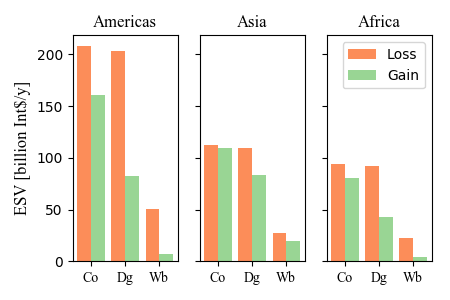
\includegraphics[scale=1]{img/esv}
%			\caption[Ecosystem service values]{}
%			\label{fig:esv}
%		\end{figure}


